\documentclass[11pt]{article}





\newcommand\CG[1]{\textcolor{red}{#1}}


\usepackage{lineno,hyperref}

\usepackage[margin=1 in]{geometry}
\renewcommand{\baselinestretch}{1.25}

\usepackage{authblk}
\usepackage{galois} % composition function \comp
\usepackage{bm}
\usepackage{amsmath}
\usepackage{amssymb}
\usepackage{mathrsfs}
\usepackage{amsthm}
\usepackage{natbib}
\usepackage{graphicx}
\usepackage{color}
\usepackage{booktabs}
\usepackage[page,title]{appendix}
%\renewcommand\appendixname{haha}
\usepackage{enumerate}
\usepackage{changepage}
\usepackage{datetime}
\newdate{date}{9}{1}{2017}

%%%%%%%%%%%%%%  Notations %%%%%%%%%%
\DeclareMathOperator{\mytr}{tr}
\DeclareMathOperator{\mydiag}{diag}
\DeclareMathOperator{\myrank}{Rank}
\DeclareMathOperator{\myP}{P}
\DeclareMathOperator{\myE}{E}
\DeclareMathOperator{\myVar}{Var}
\DeclareMathOperator*{\argmax}{arg\,max}
\DeclareMathOperator*{\argmin}{arg\,min}


\newcommand{\Ba}{\mathbf{a}}    \newcommand{\Bb}{\mathbf{b}}    \newcommand{\Bc}{\mathbf{c}}    \newcommand{\Bd}{\mathbf{d}}    \newcommand{\Be}{\mathbf{e}}    \newcommand{\Bf}{\mathbf{f}}    \newcommand{\Bg}{\mathbf{g}}    \newcommand{\Bh}{\mathbf{h}}    \newcommand{\Bi}{\mathbf{i}}    \newcommand{\Bj}{\mathbf{j}}    \newcommand{\Bk}{\mathbf{k}}    \newcommand{\Bl}{\mathbf{l}}
\newcommand{\Bm}{\mathbf{m}}    \newcommand{\Bn}{\mathbf{n}}    \newcommand{\Bo}{\mathbf{o}}    \newcommand{\Bp}{\mathbf{p}}    \newcommand{\Bq}{\mathbf{q}}    \newcommand{\Br}{\mathbf{r}}    \newcommand{\Bs}{\mathbf{s}}    \newcommand{\Bt}{\mathbf{t}}    \newcommand{\Bu}{\mathbf{u}}    \newcommand{\Bv}{\mathbf{v}}    \newcommand{\Bw}{\mathbf{w}}    \newcommand{\Bx}{\mathbf{x}}
\newcommand{\By}{\mathbf{y}}    \newcommand{\Bz}{\mathbf{z}}    
\newcommand{\BA}{\mathbf{A}}    \newcommand{\BB}{\mathbf{B}}    \newcommand{\BC}{\mathbf{C}}    \newcommand{\BD}{\mathbf{D}}    \newcommand{\BE}{\mathbf{E}}    \newcommand{\BF}{\mathbf{F}}    \newcommand{\BG}{\mathbf{G}}    \newcommand{\BH}{\mathbf{H}}    \newcommand{\BI}{\mathbf{I}}    \newcommand{\BJ}{\mathbf{J}}    \newcommand{\BK}{\mathbf{K}}    \newcommand{\BL}{\mathbf{L}}
\newcommand{\BM}{\mathbf{M}}    \newcommand{\BN}{\mathbf{N}}    \newcommand{\BO}{\mathbf{O}}    \newcommand{\BP}{\mathbf{P}}    \newcommand{\BQ}{\mathbf{Q}}    \newcommand{\BR}{\mathbf{R}}    \newcommand{\BS}{\mathbf{S}}    \newcommand{\BT}{\mathbf{T}}    \newcommand{\BU}{\mathbf{U}}    \newcommand{\BV}{\mathbf{V}}    \newcommand{\BW}{\mathbf{W}}    \newcommand{\BX}{\mathbf{X}}
\newcommand{\BY}{\mathbf{Y}}    \newcommand{\BZ}{\mathbf{Z}}    

\newcommand{\bfsym}[1]{\ensuremath{\boldsymbol{#1}}}

\def\balpha{\bfsym \alpha}
\def\bbeta{\bfsym \beta}
\def\bgamma{\bfsym \gamma}             \def\bGamma{\bfsym \Gamma}
\def\bdelta{\bfsym {\delta}}           \def\bDelta {\bfsym {\Delta}}
\def\bfeta{\bfsym {\eta}}              \def\bfEta {\bfsym {\Eta}}
\def\bmu{\bfsym {\mu}}                 \def\bMu {\bfsym {\Mu}}
\def\bnu{\bfsym {\nu}}
\def\btheta{\bfsym {\theta}}           \def\bTheta {\bfsym {\Theta}}
\def\beps{\bfsym \varepsilon}          \def\bepsilon{\bfsym \varepsilon}
\def\bsigma{\bfsym \sigma}             \def\bSigma{\bfsym \Sigma}
\def\blambda {\bfsym {\lambda}}        \def\bLambda {\bfsym {\Lambda}}
\def\bomega {\bfsym {\omega}}          \def\bOmega {\bfsym {\Omega}}
\def\brho   {\bfsym {\rho}}
\def\btau{\bfsym {\tau}}
\def\bxi{\bfsym {\xi}}
\def\bzeta{\bfsym {\zeta}}
% May add more in future.
%%%%%%%%%%%%%%%%%%%%%%%%%%%%%%%%%%%%



\theoremstyle{plain}
\newtheorem{theorem}{\quad\quad Theorem}
\newtheorem{proposition}{\quad\quad Proposition}
\newtheorem{corollary}{\quad\quad Corollary}
\newtheorem{lemma}{\quad\quad Lemma}
\newtheorem{example}{Example}
\newtheorem{assumption}{\quad\quad Assumption}
\newtheorem{condition}{\quad\quad Condition}

\theoremstyle{definition}
\newtheorem{remark}{\quad\quad Remark}
\theoremstyle{remark}


%\title{Integrated likelihood ratio test with applications to testing the homogeneity in a two-component normal mixture model}
\title{Integrated Likelihood Ratio Test}


\author[1]{Rui Wang}
\author[2]{Na Li}
\author[1,3]{Xingzhong Xu\thanks{Corresponding author\\Email address: xuxz@bit.edu.cn}}
\affil[1]{
School of Mathematics and Statistics, Beijing Institute of Technology, Beijing 
    100081,China
}
\affil[2]{
    School of Econometrics and Management, University of the Chinese Academy of Sciences, Beijing 100049, China.
}
\affil[3]{
Beijing Key Laboratory on MCAACI, Beijing Institute of Technology, Beijing 100081,China
}







\begin{document}
\maketitle
\begin{abstract}
    A general methodology named integrated likelihood ratio test is proposed which takes posterior Bayes factor and fractional Bayes factor as main test statistics.
    %Different from Bayesian hypothesis testing, we treat the resulting test procedure as a frequentist one which controls significance level.
    Under certain regular conditions, the Wilks phenomenon of the integrated likelihood ratio is proved, which can be used to determine the critical value of the test.
    We also give the asymptotic local power of the integrated likelihood ratio test.
    It is shown that the integrated likelihood ratio test shares similar frequency properties with the likelihood ratio test but requires fewer conditions.
    The integrated likelihood ratio test is available even if the likelihood functions are unbounded where the classical likelihood ratio test can not be defined.
    %However, the proposed methodology may exhibit considerable differences from likelihood ratio test.
    %Our methodology also includes the statistics produced by approximation computation.
    We apply the integrated likelihood ratio test to two submodels of the normal mixture model.
    %The normal mixture model is quite an irregular model.
    The likelihood ratio test can not be defined for the first submodel and has undesirable local power behavior for the second submodel.
    In contrast, we show that the integrated likelihood ratio test has good asymptotic power behavior for both submodels.
    %This shows that the integrated likelihood ratio test.
\end{abstract}
{\small \textsc{Keywords:} {\em
    Bayes consistency;
    Fractional posterior;
    Integrated likelihood ratio;
    Mixture model;
    Posterior Bayes factor.
    %R\'{e}nyi divergence;
   %Variational inference.
}}



\section{Introduction}

%Suppose we are interested in  testing the hypotheses $H_0:\theta\in \Theta_0$ vs. $H_1:\theta\in \Theta$ for a subset $\Theta_0$ of $\Theta$.


% Where \cite{gelfand1993bayesian} derived the null distribution of PBF.
% However, they didn't explicitly give the conditions needed. In fact, their proof relies on Laplace approximation, which assumes the existence of maximum likelihood estimator (MLE). 
% Note that the existence of MLE implies the existence of LRT. Hence the scope of their method doesn't exceed that of classical LRT\@.

%\cite{Fractional1995} proposed the fractional Bayes factor (FBF).
%The idea of fractional likelihood is also adopted by~\cite{kar10563}.
%We will see that FBF has a wider applicable scope than PBF.

%Both PBF and FBF is a special case of the general ILRT.


%Based on the proof of Bernstein-von Mises theorem (See~\cite{van2000asymptotic} and~\cite{Kleijn2012The}), we give the proof of the Wilks phenomenon and local power of ILRT under fairly weak assumptions.


%Bayesian hypothesis testing is very different from point estimation in that the data can not yanmo prior.



%%%%%% LRT %%%%%%%%%%%%%
%Likelihood ratio test (LRT) is the most widely used statistical testing method which enjoys many optimal properties.
%For example, by Neyman-Pearson lemma, it's the most powerful test in simple null and simple alternative case \citep{Lehmann}.
%In multi-dimensional parameter case, most powerful test does not exist.
%Nevertheless, the LRT is asymptotic optimal in the sense of Bahadur efficiency \citep{MR0315820}.
%However, even in some widely used models, likelihood may be unbounded. See~\cite{Cam1990Maximum} for some examples.
%In this case, LRT does not exist. Another weakness of LRT occurs when the likelihood is not concave in parameters. In this case, numerical algorithms for maximizing likelihood may trap in local maxima. 
%
Likelihood inference plays a dominant role in parametric statistic inference.
On the one hand, the maximum likelihood estimation is asymptotically optimal in a great variety of problems.
On the other hand, the fundamental lemma of Neyman and Pearson tells us that the likelihood ratio test (LRT) is the most powerful test if the null and alternative hypotheses are both simple.
For testing complex hypotheses
\begin{equation}\label{eq:newHy}
    H:\theta\in\Theta_0\quad \text{vs.}\quad K: \theta\in \Theta_1,
\end{equation}
where $\Theta_0\cap \Theta_1=\emptyset$, $\Theta_0\cup \Theta_1=\Theta$, $\Theta$ is an open subset of $\mathbb{R}^p$ and $\Theta_0$ is a $p_0$-dimensional subset of $\mathbb{R}^p$,
the LRT statistic is defined as
\begin{equation*}
    \Lambda_{\text{LRT}}=\frac{\max_{\theta\in\Theta}L(\theta)}{\max_{\theta\in\Theta_0} L(\theta)}=\frac{L(\hat{\theta}_{\text{MLE}})}{ L(\hat{\theta}^{(0)}_{\text{MLE}})},
\end{equation*}
where $L(\theta)$ is the likelihood function, $\hat{\theta}_{\text{MLE}}$ and $\hat{\theta}^{(0)}_{\text{MLE}}$ are the MLE of $\theta$ in $\Theta$ and $\Theta_0$, respectively.
A key property of the LRT is Wilks phenomenon~\citep{Wilks1938The} which asserts that for regular models, $2\log \Lambda_{\text{LRT}}$ converges to $\chi^2(p-p_0)$ in law under the null hypothesis.
The LRT has been very successful in many specific problems.
However, for some moderately complex problems, some difficulties may arise when using the LRT.
The maximization of $L(\theta)$ may be difficult if the likelihood function is not concave and has multiple local maxima.
Worse still, in some problems the likelihood functions are unbounded and hence the LRT is not defined; see, for example,~\cite{Cam1990Maximum}.
Notice that the unbounded likelihood occurs not only in artificial models, but also in some widely used models, such as the mixture models with unknown component location and scale parameters~\citep{chenjiahua2017}.

In goodness of fit test, there are two common types of tests: extreme value type (Kolmogorov-Smirnov test, e.g.) and integral type (Cram\'er-von Mises test, e.g.).
In classical parametric hypothesis testing, however, no attention has been paid to the integrated likelihood functions.
A natural integral type test statistic for hypothesis \eqref{eq:newHy} is
\begin{equation}\label{naiLiS}
\frac{\int_{\Theta}L(\theta) d\Pi(\theta)}{\int_{\Theta_0} L(\theta) d\Pi^{(0)}(\theta)},
\end{equation}
where $\Pi$ and $\Pi^{(0)}$ are some probability measures on $\Theta$ and $\Theta_{0}$, respectively.
If $\Pi$ and $\Pi^{(0)}$ are independent of data, then the statistic~\eqref{naiLiS} is exactly the Bayes factor \citep{scientificInference} with the prior distributions $\Pi$ and $\Pi^{(0)}$.
The Bayes factor is the conventional tool for Bayesian hypothesis testing and has been widely used by practitioners; see~\cite{Robert1995Bayes} for a review.
%Compared with other aspects of Bayesian inference, % such as point estimation and credible sets,
%Bayes factor is developed on its own ground. % and thus has its own nature.
%Bayes factor can not be obtained solely from the posterior distribution of parameters.
%There are two consequence of this feature.
%First, the computation of Bayes factor is highly nontrivial;see~\cite{Robert1995Bayes},~\cite{MarkovC},~\cite{raftery2006estimating} and the references therein.
However, Bayes factor is sensitive to the choice of prior distribution. 
In fact, the asymptotic distribution of Bayes factor depends on the prior density at the true parameter; see, for example,~\cite{clarke1990information}.
As a result, the Bayes factor cannot be treated as a frequentist test statistic.
Thus, the measures $\Pi$ and $\Pi^{(0)}$ considered in this paper will depend on data.
%\CG{As a special case, $\Pi$ and $\Pi^{(0)}$ can be posterior distributions.}

If $\Pi(\theta=\hat{\theta}_{\text{MLE}})=1$ and $\Pi^{(0)}(\theta=\hat{\theta}^{(0)}_{\text{MLE}})=1$, then the statistic~\eqref{naiLiS} becomes the LRT statistic.
In this case, the measure $\Pi$ and $\Pi^{(0)}$ both concentrate on one point and are highly nonsmooth.
For many models where the LRT fails, the likelihood function $L(\theta)$ still has good properties for most $\theta$ and  the MLE is unfortunately trapped in a fairly small area of $\theta$ where $L(\theta)$ has bad behavior.
Figure~\ref{myFigure1} exhibits this phenomenon.
%In such cases, some smoother $\Pi$ and $\Pi^{(0)}$ may perform better intuitively.
Intuitively,
if $\Pi$ and $\Pi^{(0)}$ are smooth and have small tail probability,
then the defeat of the likelihood function in a small area will not introduce much effect on the integrated likelihood.
Following this idea, a natural choice is to take $\Pi$ and $\Pi^{(0)}$ as the posterior distribution (with certain prior distributions) of $\theta$ in $\Theta$ and $\Theta_0$, respectively.
In this case, the statistic~\eqref{naiLiS} becomes the posterior Bayes factor proposed (PBF) by~\cite{Aitkin1991Posterior}.
~\cite{Aitkin1991Posterior} argued that if the likelihood is concentrated around the MLE, the PBF should approximately equal to $2^{(p-p_0)/2}\Lambda_{\text{LRT}}$.
This implies that PBF has the similar Wilks phenomenon as the LRT.
%Note that if the likelihood is concentrated around the MLE, then the MLE is consistent and thus the LRT can be applied.
%Hence we are more interested in the case where the MLE is inconsistent.
%In a theoretical point of view, the Wilks phenomenon of PBF requires certain conditions which are undesirable.
%In contrast, it is well known that the posterior distribution tends to become independent of the prior distribution as the sample size increases.
%Several modifications of Bayes factor have been proposed.

\begin{figure}
    \begin{center}
        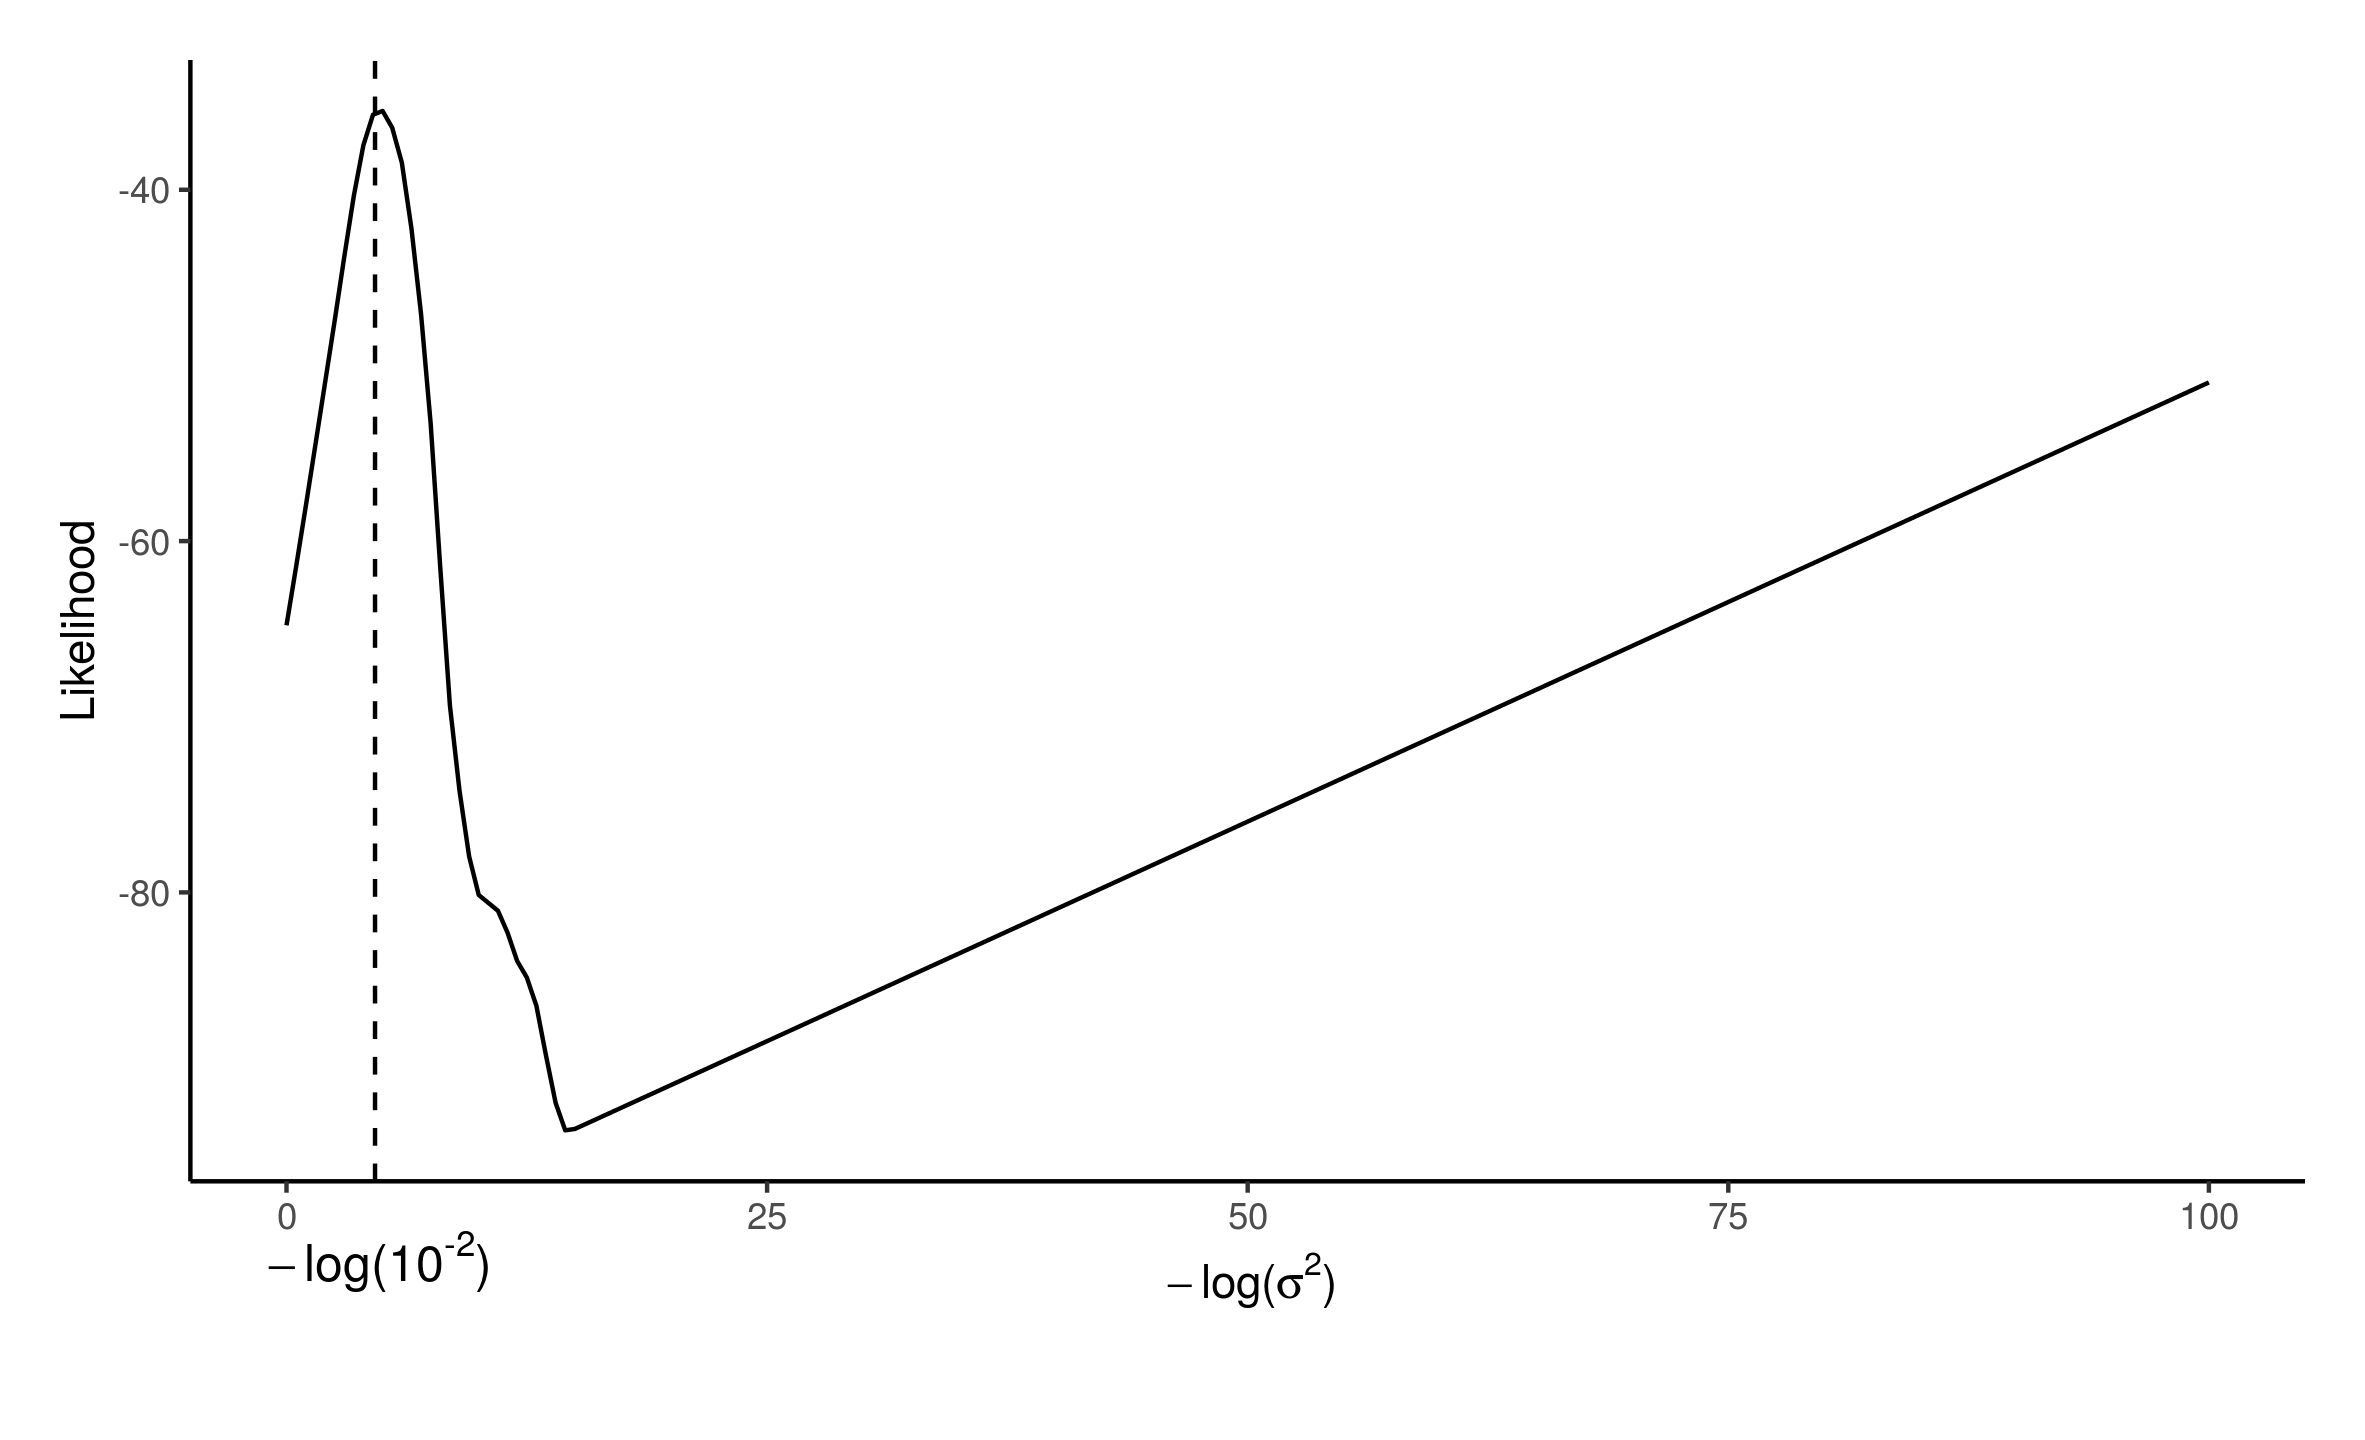
\includegraphics[width=0.9\textwidth]{figure/newnewPP}
    \end{center}
    \caption{
        An example of unbounded likelihood.
        We data $X_1,\ldots,X_n$ which are iid from the mixture model $(1-\omega)\mathcal{N}(0,1)+\omega\mathcal{N}(\xi,\sigma^2)$ with $(\omega,\xi,\sigma^2)^T=(1/2,1,10^{-2})$ and $n=50$.
        We plot the likelihood function  in $-\log (\sigma^2)$ with $\omega=1/2$ and $\xi=X_1$.
        The likelihood tends to infinity as $-\log (\sigma^2)$ tends to infinity, i.e., $\sigma^2$ tends to $0$.
        In contrast, the likelihood has a local maximum around the true parameter $-\log (\sigma^{2})=-\log (10^{-2})$.
    }
    \label{myFigure1}
\end{figure}



If we replace the likelihood function $L(\theta)$ by $L(\theta)^a$ for $a>0$, then the LRT statistic becomes
\begin{equation*}
    \frac{\max_{\theta\in\Theta}L^{a}(\theta)}{\max_{\theta\in\Theta_0}L^a(\theta)}=\Lambda^a_{\text{LRT}},
\end{equation*}
%Hence the LRT statistic is equivariant if we raise the likelihood to the power of $a$.
which is equivalent to the LRT statistic.
In contrast, the statistic
\begin{equation}\label{naiLiS2}
\frac{\int_{\Theta}L^a(\theta) d\Pi(\theta)}{\int_{\Theta_0} L^a(\theta) d\Pi^{(0)}(\theta)}
\end{equation}
is not equivalent to the statistic~\eqref{naiLiS}.
We will also consider the test statistic~\eqref{naiLiS2} with $0<a<1$.
Correspondingly, the measure $\Pi$ and $\Pi^{(0)}$ can also take the fractional posterior~\citep{Bha2016}.
Raising the likelihood to a fractional power has several advantages; see, e.g.,~\cite{kar10563} and~\cite{Bha2016}.
In particular, the consistency of the fractional posterior requires less conditions than the consistency of the usual posterior.
A special case of the statistic~\eqref{naiLiS2} is the fractional Bayes factor (FBF) proposed by \cite{Fractional1995}.
We call the statistic~\eqref{naiLiS2} the generalized FBF if $\Pi$ and $\Pi^{(0)}$ are fractional posterior distributions.

Under certain regular conditions, we rigorously prove the Wilks phenomenon of the generalized FBF.
Based on the Wilks phenomenon, an asymptotically correct frequentist test procedure can be formulated.
We also give the asymptotic local power of the resulting test procedure under contiguous alternative.
It is shown that the generalized FBF has a similar asymptotic local power to the LRT.
However, the generalized FBF
can be applied to the cases where the likelihood is unbounded
and thus has a wider application scope than the LRT.


%The frequentist properties of Bayesian methods have drawn much attention in recent years.
%See~\cite{ghosal2000},~\cite{Shen2001Rates},~\cite{vaart2007convergence},~\cite{Kleijn2012The} and the references therein.
%These works show that many Bayesian methods still perform well when they are treated as frequentist methods.
%%However, existing research is largely concerned with the consistency and asymptotic normality of the posterior distribution.
%Existing research is largely concerned with the frequentist properties of Bayesian point estimation and credible sets.
%For these problems, Bayesian methods can be directly treated as frequentist methods.
%However, for testing problem, Bayesian methods are not required to control the type I error rate and hence can not be directly treated as frequentist methods.

%Compared with likelihood ratio test which utilize the maximum of the likelihood, Bayesian methods integrate the likelihood by a weight function.
%Can these Bayesian methods be formulated into frequentist tests?
%If they can, what's the behavior of these tests?
%This paper is devoted to answering such questions.

%Motivated by this, we propose a flexible methodology called integrated likelihood ratio test (ILRT) which takes PBF and FBF as special examples.
%ILRT also includes methods that are produced by approximation computation.



The generalized FBF can be computed by sampling $\theta$ from the fractional posterior and calculate the sample mean of the fractional likelihood.
For moderately complex model, however, sampling from the fractional posterior may be difficult and hence some approximation methods may be used in practice.
%The computations of PBF and FBF are easier than that of Bayes factor since the PBF and FBF can be computed by sampling the likelihood according to posterior distribution or fractional posterior distribution.
Variational inference is a popular method for approximating intractable posterior distribution; see~\cite{blei2017} and the references therein.
Such procedure produces a distribution other than the fractional posterior distribution.
To accommodate such cases, we also give a theorem (Theorem~\ref{theoremMain} in Section 2) for the general measure $\Pi$ and $\Pi^{(0)}$ in~\eqref{naiLiS2}.
%{\color{red} Allow $a+b=1$.}





For some irregular problems, the behavior of likelihood is complicated.
%Since the integral of the likelihood can smooth the irregular behavior of the likelihood, it can be expected that ILRT may have better behavior than the LRT.
%To illustrate this point,
We apply the proposed method to testing the homogeneity in a two-component normal mixture model.
This problem is fairly irregular and suffers from nonidentifiability and nonconcave likelihood.
~\cite{HALL2005158} showed that the likelihood ratio test has trivial power under $n^{-1/2}$ local alternative hypothesis. 
In contrary, we show that the ILRT have nontrivial power under $n^{-1/2}$ local alternative hypothesis.



The paper is organized as follow.
In Section 2, we prove the Wilks phenomenon of the ILRT statistic and gives the asymptotic local power of the corresponding test.
In Section 3, we apply ILRT to testing the homogeneity in a two-component normal mixture model.
Section 4 concludes the paper.
All technical proofs are in Appendix.





\section{Integrated likelihood ratio test}

\subsection{The test statistic}

Let $\BX^{(n)}=(X_1,\ldots,X_n)$ be independent identically distributed (iid) observations taking values in some space $(\mathcal{X};\mathscr{A})$.
Suppose that there is a $\sigma$-finite measure $\mu$ on $\mathcal{X}$ and that the  possible distribution $P_\theta$ of $X_i$ has a density $p(X|\theta)$ with respect to $\mu$.
Denote by $P_{\theta}^{n}$ the joint distribution of $\BX^{(n)}$.
Let $p_{n}(\BX^{(n)}|\theta)=\prod_{i=1}^n p(X_i|\theta)$ denote the density of $P_{\theta}^n$ with respect to the $n$-fold product measure $\mu^n$.
The parameter $\theta$ takes its values in $\Theta$, an open subset of $\mathbb{R}^{p}$.
Suppose $\theta=(\nu^T,\xi^T)^T$, where $\nu$ is a $p_0$ dimensional subvector and $\xi$ is a $p-p_0$ dimensional subvector.
 We would like to test the hypotheses
\begin{equation*}
    H:\theta\in\Theta_0\quad \text{v.s.}\quad K:\theta\in\Theta\backslash \Theta_0,
\end{equation*}
where the null space $\Theta_0$ is a $p_0$-dimensional subspace of $\Theta$ defined as
\begin{equation*}
    \Theta_0=\{(\nu^T,\xi^T)^T:(\nu^T,\xi^T)^T\in\Theta, \, \xi=\xi_0\}.
\end{equation*}
If the null hypothesis is true, we denote by $\theta_0=(\nu_0^T,\xi_0^T)^T$ the true parameter which generates the data.



%The conventional Bayes factor is defined as
%\begin{equation*}
  %\frac{\int_{\Theta} p_n(\BX^{(n)}|\theta)\pi(\theta)\, d\theta}
    %{\int_{\tilde{\Theta}_0}p_n(\BX^{(n)}|\nu,\xi_0)\pi(\nu)\, d\nu},
%\end{equation*}
%where $\tilde{\Theta}_0=\{\nu: (\nu^T,\xi^T)^T\in \Theta_0\}$.
%However, Bayes factor is sensitive to the specification of prior, which may cause difficulties in the absence of a well-formulated subjective prior; see, e.g., \cite{Lindley1982}.
%The frequency property of Bayes factor is not satisfactory.
%To overcome this weakness, several robust alternatives to Bayes factor have been proposed.
%To deal with this problem,
In Bayesian hypothesis testing framework, one puts prior $\pi(\nu)$ and $\pi(\theta)$ on parameters under the null and alternative hypotheses, respectively.
The PBF proposed by~\cite{Aitkin1991Posterior}  is defined as
\begin{equation*}
    \frac{\int_{\Theta} p_n(\BX^{(n)}|\theta)\pi(\theta|\BX^{(n)})\, d\theta}{\int_{\tilde{\Theta}_0}p_n(\BX^{(n)}|\nu,\xi_0)\pi(\nu|\BX^{(n)})\, d\nu},
\end{equation*}
where
$\tilde{\Theta}_0=\{\nu: (\nu^T,\xi^T)^T\in \Theta_0\}$, $\pi(\nu|\BX^{(n)})$ and $\pi(\theta|\BX^{(n)})$ are the posterior densities under the null and alternative hypothesis, respectively.
The FBF proposed by~\cite{Fractional1995} is defined as
\begin{equation*}
    \frac{L_{1}(\Theta;\BX^{(n)})}{L_{b}(\Theta;\BX^{(n)})}\cdot \frac{L_{b}^{(0)}(\tilde{\Theta}_0;\BX^{(n)})}{L_{1}^{(0)}(\tilde{\Theta}_0;\BX^{(n)})}\quad \text{for}\quad 0<b<1,
\end{equation*}
where for $t>0$ and sets $A\subset \Theta$, $A_0\subset \tilde{\Theta}_0$,
 $$
 L_t(A;\BX^{(n)})=\int_{A}\big[p_n(\BX^{(n)}|\theta)\big]^t \pi(\theta)\, d\theta,\quad
 L_t^{(0)}(A_0;\BX^{(n)})=\int_{A_0}\big[p_n(\BX^{(n)}|\nu,\xi_0)\big]^t \pi(\nu)\, d\nu.
 $$

 Being treated as frequentist test statistics, the PBF and FBF are both integrated type statistics.
 We generalize the PBF and FBF and propose the following integrated likelihood ratio test statistic
\begin{equation*}
    \frac{\int_{\Theta} \big[p_n(\BX^{(n)}|\theta)\big]^{a}\pi(\theta;\BX^{(n)})\,d\theta}{\int_{\tilde{\Theta}_0} \big[p_n(\BX^{(n)}|\nu,\xi_0)\big]^{a}\pi(\nu;\BX^{(n)})\,d\nu},
\end{equation*}
where $a>0$ is a hyperparameter,
the weight functions $\pi(\theta;\BX^{(n)})$ and $\pi(\nu;\BX^{(n)})$ are probability density functions in $\Theta$ and $\tilde{\Theta}_0$ given $\BX^{(n)}$, respectively.
Note that $\pi(\theta;\BX^{(n)})$ and $\pi(\nu;\BX^{(n)})$ are data dependent but does not need to be the posterior density.

If we take the weight function as the fractional posterior
\begin{equation}\label{firstWeight}
\pi(\theta;\BX^{(n)})=\frac{\big[p_n(\BX^{(n)}|\theta)\big]^b \pi(\theta)}{\int_{\Theta}\big[p_n(\BX^{(n)}|\theta)\big]^b \pi(\theta)\, d\theta},
\quad
\pi(\nu;\BX^{(n)})=\frac{\big[p_n(\BX^{(n)}|\nu,
    \xi_0)\big]^b \pi(\nu)}{\int_{\tilde{\Theta}_0}\big[p_n(\BX^{(n)}|\nu,\xi_0)\big]^b \pi(\nu)\, d\nu},
\end{equation}
then the ILRT statistic equals to
$$
    \Lambda_{a,b}=
    \frac{L_{a+b}(\Theta;\BX^{(n)})}{L_{b}(\Theta;\BX^{(n)})}\cdot \frac{L_{b}^{(0)}(\tilde{\Theta}_0;\BX^{(n)})}{L_{a+b}^{(0)}(\tilde{\Theta}_0;\BX^{(n)})}.
$$
We call $\Lambda_{a,b}$ the generalized FBF throughout the paper.
The FBF and PBF are both the special cases of the generalized FBF.
In fact, the FBF equals to $\Lambda_{1-b,b}$, the PBF equals to $\Lambda_{1,1}$.
For some moderately complex models, the fractional posterior~\eqref{firstWeight} may be complicated.
%Consequently, sampling from~\eqref{firstWeight} may be intractable.
In this case, one may use some simple form weight function to approximate the fractional posterior~\eqref{firstWeight}.
A popular method for approximating~\eqref{firstWeight} is variational inference;
see, e.g.,~\cite{blei2017}.
In this case, the weight function in~\eqref{eq:definition} is equals to the variational approximation of~\eqref{firstWeight}.
The ILRT methodology also includes such approximate method.

The computation of the ILRT statistic is relatively simple.
We can independently generate $\theta_1,\ldots,\theta_m$ and $\nu_1,\ldots,\nu_m$ according to $\pi(\theta;\BX^{(n)})$ and $\pi(\nu;\BX^{(n)})$ for a large $m$.
Then the ILRT statistic can be approximated by
\begin{equation*}
    \frac{\sum_{i=1}^m \big[p_n(\BX^{(n)}|\theta_i)\big]^{a}}{\sum_{i=1}^m\big[p_n(\BX^{(n)}|\nu_i,\xi_0)\big]^{a}}.
\end{equation*}




\subsection{Generalized FBF}
In this section, we investigate the asymptotic behavior of the generalized FBF.
The following assumption is adapted from~\cite{Kleijn2012The} and is satisfied by many common models. 
%The function $\theta \mapsto \log p(X|\theta)$ is differentiable at $\theta_0$  $P_{\theta_0}$-a.s.\ with derivative 
%$$\dot{\ell}_{\theta_0}(X)=\frac{\partial}{\partial \theta}\log p(X|\theta)\Big|_{\theta=\theta_0}.$$
%There's an open neighborhood $V$ of $\theta_0$ such that for every $\theta_1,\theta_2\in V$,
        %\begin{equation*}
            %|\log p(X|\theta_1)-\log p(X|\theta_2)|\leq m(X)\|\theta_1-\theta_2\|,
        %\end{equation*}
        %where $m(X)$ is a measurable function satisfying $P_{0}\exp[s m(X)]<\infty$ for some $s>0$.
        %The Fisher information matrix $I_{\theta_0}=P_{\theta_0}\dot{\ell}_{\theta_0}\dot{\ell}_{\theta_0}^T$ is positive-definite and as $\theta\to \theta_0$,
    %\begin{equation*}
        %P_{\theta_0} \log \frac{p(X|\theta)}{ p(X|\theta_0)}
        %=-\frac{1}{2}(\theta-\theta_0)^T I_{\theta_0} (\theta-\theta_0)+o(\|\theta-\theta_0\|^2).
    %\end{equation*}
\begin{assumption}\label{Assumption1}
    The parameter spaces $\Theta$ and $\tilde{\Theta}_0$ are open subsets of $\mathbb{R}^p$ and $\mathbb{R}^{p_0}$, respectively.
    The parameters $\theta_0$ and $\nu_0$ are inner points of $\Theta$ and $\tilde{\Theta}_0$, respectively.
    The derivative 
$$\dot{\ell}_{\theta_0}(X)=\frac{\partial}{\partial \theta}\log p(X|\theta)\Big|_{\theta=\theta_0}$$
exists $P_{\theta_0}$-a.s.\ and satisfies $P_{\theta_0}\dot{\ell}_{\theta_0}=0_p$.
The Fisher information matrix $I_{\theta_0}=P_{\theta_0}\dot{\ell}_{\theta_0}\dot{\ell}_{\theta_0}^T$ is positive-definite, where $P f$ means the expectation of $f(X)$ when $X$ has distribution $P$.
For every $M>0$,
    \begin{equation*}
        \sup_{\|h\|\leq M}\Big|
         \log \frac{p_n(\BX^{(n)}|\theta_0+n^{-1/2}h)}{p_n(\BX^{(n)}|\theta_0)}-h^T I_{\theta_0}\Delta_{n,\theta_0}+\frac{1}{2}h^T I_{\theta_0}h
         \Big|\xrightarrow{P^n_{\theta_0}}0,
    \end{equation*}
    where $\Delta_{n,\theta_0}=n^{-1/2}\sum_{i=1}^n I_{\theta_0}^{-1}\dot{\ell}_{\theta_0}(X_i)$.
\end{assumption}     
%, it ensures a local asymptotic normality expansion of likelihood. See Lemma~\ref{Thm:localExpansion} in Appendix.
For $t>0$, we say $L_t(\cdot;\BX^{(n)})$ is $\sqrt{n}$-consistent if for every $M_n\to \infty$,
    $$
    \frac{L_t({\{\theta:\|\theta-\theta_0\|> M_n/\sqrt{n}\}};\BX^{(n)})}{L_t(\Theta;\BX^{(n)})}\xrightarrow{P_{\theta_0}^n} 0.
    $$
    The $\sqrt{n}$-consistency of $L_t^{(0)}(\cdot;\BX^{(n)})$ is similarly defined.
    Note that the consistency of $L_1(\cdot;\BX^{(n)})$ is equivalent to the consistency of the posterior distribution.
    In~\cite{Kleijn2012The}, the $\sqrt{n}$-consistency of posterior distribution is a key assumption to prove Bernstein-von Mises theorem.
    Likewise, the $\sqrt{n}$-consistency of $L_t(\cdot;\BX^{(n)})$ is a key assumption of the following theorem.



    \begin{theorem}\label{Thm:maintheorem}
        Suppose that Assumption~\ref{Assumption1} holds, $L_{a+b}(\cdot;\BX^{(n)})$, $L_b(\cdot;\BX^{(n)})$, $L_{a+b}^{(0)}(\cdot;\BX^{(n)})$ and $L_b^{(0)}(\cdot;\BX^{(n)})$ are $\sqrt{n}$-consistent, $\pi(\theta)$ is continuous at $\theta_0$ with $\pi(\theta_0)>0$, $\pi(\nu)$ is continuous at $\nu_0$ with $\pi(\nu_0)>0$. Then for $\{\theta_n\}$ such that $\sqrt{n}(\theta_n-\theta_0)\to \eta$, 
        $$
        2\log \Lambda_{a,b}\overset{P^n_{\theta_n}}{\rightsquigarrow}-{(p-p_0)}\log (1+\frac{a}{b})+{a}\chi^2(p-p_0,\delta),
        $$
        where $\chi^2(p-p_0,\delta)$ is a noncentral chi-squared random variable with $p-p_0$ degrees of freedom and noncentrality parameter $\delta=\eta^T\big( I_{\theta_0}-I_{\theta_0} J(J^T I_{\theta_0} J)^{-1}J^T I_{\theta_0}\big)\eta$ and $J=(I_{p_0},0_{p_0\times(p-p_0)})^T$,
``$\rightsquigarrow$'' means weak convergence.
    \end{theorem}
Theorem~\ref{Thm:maintheorem} gives the asymptotic distribution of $2\log \Lambda_{a,b}$ under the null hypothesis and the local alternative hypothesis.
To formulate a test with asymptotic type I error rate $\alpha$, the critical value of $2\log \Lambda_{a,b}$ can be defined to be $-(p-p_0)\log (1+a/b)+ a\chi^2_{1-\alpha}(p-p_0)$ where $\chi^2_{1-\alpha}(p-p_0)$ is the $1-\alpha$ quantile of a chi-squared random variable with $p-p_0$ degrees of freedom.
By Theorem~\ref{Thm:maintheorem}, the resulting test has local asymptotic power
\begin{equation}\label{eq:likelihoodPower}
\Pr \left( \chi^2(p-p_0,\delta)> \chi^2_{1-\alpha}(p-p_0) \right).
\end{equation}
It is known that, under certain regular conditions,~\eqref{eq:likelihoodPower} is also the local asymptotic power of the likelihood ratio test. 
In this view, $\Lambda_{a,b}$ enjoys good frequentist properties.


 The $\sqrt{n}$-consistency of $L_t(\cdot;\BX^{(n)})$ is a key assumption of Theorem \ref{Thm:maintheorem}.
Hence we would like to give sufficient conditions for the $\sqrt{n}$-consistency of $L_t(\cdot;\BX^{(n)})$.
 First we consider the exponential family of distributions.
\begin{proposition}\label{exponentialCon}
    Suppose $p(X|\theta)=\exp\big[\theta^T T(X)-A(\theta)\big]$, $\Theta$ is an open subset of $\mathbb{R}^p$, $\theta_0$ is an interior point of $\Theta$, 
    $$I_{\theta_0}=\frac{\partial^2}{\partial \theta \partial \theta^T} A(\theta_0)>0.$$
    Then $L_{t}(\cdot;\BX^{(n)})$ is consistent for $t>0$.
\end{proposition}

Proposition~\ref{exponentialCon} establishes the $\sqrt{n}$-consistent of $L_t(\cdot;\BX^{(n)})$ for all $t>0$ under full-rank exponential family models.
If the full model and the null model both belong to the full-rank exponential family, Assumption~\ref{Assumption1} is also satisfied.
%In this case, Theorem~\ref{Thm:maintheorem} implies that the generalized FBF can be used as frequentist test.
Hence, Theorem~\ref{Thm:maintheorem} implies that the generalized FBF has the similar asymptotic properties with the classical LRT statistic.
However,
for any test methodology, the success in the full-rank exponential family models is just a minimal requirement 
since the LRT is also easy to implement and enjoys good asymptotic properties.
We would like to consider more general models.


For general models, the likelihood function may not be concave.
This often makes it hard to implement the LRT.
For some models, a more serious problem may occur, that is, the likelihood may be unbounded and hence the LRT can not be defined.
This problem may occur even if the likelihood function has good local analytical properties, such as location-scale mixture models.  See \cite{Cam1990Maximum} for more examples.
A natural question is that if the fractional integrated likelihood $L_t(\Theta;\BX^{(n)})$ is always well defined.
The following theorem shows that $L_t(\Theta;\BX^{(n)})$ is always well defined for $t\leq 1$ and is not well defined for some model for $t>1$.
%For more general models, however, the $\sqrt{n}$-consistency of $L_t$ needs further conditions.
%For more general models, however, the $\sqrt{n}$-consistency of $L_t$ is more complicated.
\begin{proposition}
    If $t\leq 1$, $L_t(\Theta;\BX^{(n)})< +\infty$ $P_{\theta_0}^n$-a.s. for any models. If $t> 1$, $L_t(\Theta;\BX^{(n)}) = +\infty$ for some models.
    \label{exprop}
\end{proposition}


%It turns out that the behavior of $L_t$ for $t>1$ and $t\leq 1$ are different.

Because of the bad behavior of $L_t(\Theta;\BX^{(n)})$ for $t>1$, next we only consider $L_t(\Theta;\BX^{(n)})$ for $t\leq 1$.
For $t=1$, the $\sqrt{n}$-consistency of $L_t(\cdot;\BX^{(n)})$ is equivalent to the $\sqrt{n}$-consistency of the posterior distribution which is a well studied problem; see, e.g.,~\cite{ghosal2000},~\cite{Shen2001Rates},~\cite{vaart2007convergence}.
A popular and convenient way of establishing the consistency of posterior is through the condition that suitable test sequences exist.
This approach is adopted by~\cite{ghosal2000},~\cite{vaart2007convergence} and~\cite{Kleijn2012The}.
For example, Theorem 3.1 of \cite{Kleijn2012The} assumes that for every $\epsilon>0$, there exists a sequence of tests $\phi_n$ such that
\begin{equation}\label{eq:testSeq}
    P_{\theta_0}^n\phi_n\to 0,\quad \sup_{\|\theta-\theta_0\|\geq \epsilon} P_\theta^n(1-\phi_n)\to 0.
\end{equation}
This condition is satisfied when the parameter space is compact and the model is suitably continuous; see Theorem 3.2 of~\cite{Kleijn2012The}.
However, if the parameter space is not compact, one may have to manually construct a test sequence satisfying the condition~\eqref{eq:testSeq}.

%\begin{proposition}[\cite{Kleijn2012The}, Theorem 3.1]
    %Suppose $\theta_0$ is an interior of $\Theta$, $\pi(\theta)$ is continuous at $\theta_0$ and $\pi(\theta_0)>0$.
    %Under Assumptions \ref{Assumption1} and~\ref{Assumption2}, $L_1$ is consistent.
%\end{proposition}


%The consistency of $L_t$ for $t>1$ can be proved under conditions similar to Assumption~\ref{Assumption2}.
%However, the requirement on the sequence $\{\phi_n\}$ lacks statistical interpretation for $t>1$.



The consistency of $L_t(\cdot;\BX^{(n)})$ for $0<t<1$ is different from $t=1$.
\cite{kar10563} considered the Hellinger consistency of $L_{1/2}(\cdot;\BX^{(n)})$.
They derived the consistency of $L_{1/2}(\cdot;\BX^{(n)})$ under simple conditions.
%They only consider $t=1/2$ and didn't consider the $\sqrt{n}$-convergence result.
Recently,~\cite{Bha2016} further developed the idea of~\cite{kar10563} and derived a general bounds for the consistency of $L_t(\cdot;\BX^{(n)})$ for $0<t<1$.
However, their result can not yield the $\sqrt{n}$-consistency for parametric models.
We shall prove the $\sqrt{n}$-consistency of $L_{t}(\cdot;\BX^{(n)})$ for $0<t<1$ under certain conditions on the R\'{e}nyi divergence between distributions in the family $\{P_\theta:\theta\in\Theta\}$.

 For two parameters $\theta_1$ and $\theta_2$, the $\alpha$ order R\'{e}nyi divergence ($0<\alpha<1$) of $P_{\theta_1}$ from $P_{\theta_2}$ is defined to be
$$
D_{\alpha}(\theta_1||\theta_2)=-\frac{1}{1-\alpha}\log \rho_{\alpha}(\theta_1,\theta_2),
$$
where
$
\rho_{\alpha}(\theta_1,\theta_2)=\int_{\mathcal{X}} p(X|\theta_1)^{\alpha} p(X|\theta_2)^{1-\alpha} \, d \mu
$ is the so-called Hellinger integral.
The following assumption is needed for our $\sqrt{n}$-consistency result.
\begin{assumption}\label{Assumption4}
    For some $\alpha\in(0,1)$, there exist positive constants $\delta$, $\epsilon$ and $C$ such that,
     $D_{\alpha}(\theta||\theta_0)  \geq  C \|\theta-\theta_0\|^2$ for $\|\theta-\theta_0\|\leq \delta$ and $D_{\alpha}(\theta||\theta_0) \geq \epsilon$ for $\|\theta-\theta_0\|>\delta$.
\end{assumption}
\begin{remark}
    A remarkable property of R\'{e}nyi divergence is the equivalence of all $D_{\alpha}$: If $0<\alpha<\beta<1$, then
    $$
    \frac{\alpha}{1-\alpha}\frac{1-\beta}{\beta} D_{\beta}(\theta_1||\theta_2)
    \leq D_{\alpha}(\theta_1||\theta_2)\leq D_{\beta}(\theta_1||\theta_2).
    $$
    See, e.g.,~\cite{2016arXiv160801805B}.
    As a result, if Assumption~\ref{Assumption4} holds for some $\alpha\in(0,1)$, then it will hold for every $\alpha\in(0,1)$.
\end{remark}
To appreciate Assumption~\ref{Assumption4},
   suppose, for example, that $D_{\alpha}(\theta||\theta_0)$ is twice continuously differentiable in $\theta$.
   Since $\theta=\theta_0$ is a minimum point of  $D_{\alpha}(\theta||\theta_0)$, the first order derivative of $D_{\alpha}(\theta||\theta)$ at $\theta=\theta_0$ is zero and the second order derivative at $\theta=\theta_0$ is positive semidefinite.
By Taylor theorem, in a small neighbourhood of $\theta_0$,
   $$
   D_{\alpha}(\theta||\theta_0)=\frac{1}{2}(\theta-\theta_0)^T \frac{\partial^2}{\partial \theta \partial \theta^T} D_{\alpha}(\theta||\theta_0)\Big|_{\theta=\theta^*}  (\theta-\theta_0),
   $$
   where $\theta^*$ is between $\theta_0$ and $\theta$.
   If we further assume the second order derivative is positive definite at $\theta=\theta_0$, then in a small neighbourhood of $\theta_0$, there is a positive constant $C$ such that $D_{\alpha}(\theta||\theta_0)\geq C\|\theta-\theta_0\|^2$.
Thus, Assumption~\ref{Assumption4} is a fairly weak condition.
%It is often straightforward to verify Assumption~\ref{Assumption4}.
%Compared with Assumption~\ref{Assumption2},
%%%%%%%%%%%%%%% Here we haven't consider the second condition. It can be done through a minimax lower bound argument.
\begin{proposition}\label{Theoremless1}
    Suppose $\theta_0$ is an interior of $\Theta$, $\pi(\theta)$ is continuous at $\theta_0$ and $\pi(\theta_0)>0$.
    Under Assumptions \ref{Assumption1} and~\ref{Assumption4}, for fixed $t\in(0,1)$, $L_t(\cdot;\BX^{(n)})$ is consistent.
\end{proposition}
Note that if the conditions of Theorem~\ref{Thm:maintheorem} are satisfied, the asymptotic power of $\Lambda_{a,b}$ is independent of $a,b$.
Hence specific choices of $a,b$ are not crucial provided $L_{a+b}(\cdot;\BX^{(n)})$, $L_b(\cdot;\BX^{(n)})$, $L^{(0)}_{a+b}(\cdot;\BX^{(n)})$ and $L^{(0)}_b(\cdot;\BX^{(n)})$ are $\sqrt{n}$-consistent.
For some models, it is more convenient to verify Assumption~\ref{Assumption4} than to directly construct a test sequence satisfying the condition~\eqref{eq:testSeq}.
In such cases, it can be recommended to use the generalized FBF with $a+b< 1$.
%By Theorem~\ref{Thm:maintheorem} and Proposition~\ref{Theoremless1}, one can .


\subsection{General weight function}
For some moderately complex models, the fractional posterior~\eqref{firstWeight} are not easy to calculate.
In such cases, one may want to use simpler weight functions to approximate~\eqref{firstWeight}.
In this section, we consider the asymptotic properties of the ILRT statistic with general weight functions.

Let $h=\sqrt{n}(\theta-\theta_0)$ be the local parameter and $\pi_n(h;\BX^{(n)})=\pi(\theta_0+n^{-1/2}h;\BX^{(n)})$ be the weight function in terms of $h$.
%Then the posterior density of $h$ is $\pi_n(h|\BX^{(n)})=n^{-1/2}\pi(\theta|\BX^{(n)})$.
%Theorem 2.1 of \cite{Kleijn2012The},
If $\pi(\theta;\BX^{(n)})$ is the posterior density of $\theta$, then Bernstein-von Mises theorem asserts that under certain conditions,
$
            \|\pi_n(h;\BX^{(n)})-\phi(h;\Delta_{n,\theta_0},I_{\theta_0}^{-1})\|
$
converges to $0$ in $P_{\theta_0}^n$ probability,
where for two densities $q_1(h)$ and $q_2(h)$, $\|q_1(h)-q_2(h)\|=\int |q_1(h)-q_2(h)|\, dh$ is their total variation distance.
Similarly, if $\pi(\theta;\BX^{(n)})$ is the fractional posterior density of $\theta$ with fractional power $b$, it can be proved that under certain conditions,
$
\|\pi_n(h;\BX^{(n)})-\phi(h;\Delta_{n,\theta_0},b^{-1} I_{\theta_0}^{-1})\|
$
converges to $0$ in $P_{\theta_0}^n$ probability.
We shall assume that the weight function inherits such properties.
        
\begin{assumption}\label{Assumption3}
    Let $b\in(0,1)$ be a fixed number.
    Assume that $\pi_n(h;\BX^{(n)})$ satisfies
        \begin{equation}\label{vonMisesResults}
            \|\pi_n(h;\BX^{(n)})-\phi(h;\Delta_{n,\theta_0},b^{-1}I_{\theta_0}^{-1})\|\overset{P_{\theta_0}^n}{\to}0.
        \end{equation}

        Similarly, let $h^{(0)}=\sqrt{n}(\nu-\nu_0)$. Define $\pi_n(h^{(0)};\BX^{(n)})=n^{-1/2}\pi(\nu;\BX^{(n)})$. Assume that 
\begin{equation}\label{vonMisesResultsl}
    \|\pi_n(h^{(0)};\BX^{(n)})-\phi(h^{(0)};\Delta^{(0)}_{n,\theta_0},b^{-1}I_{\theta_0}^{(0)-1})\|\overset{P_{\theta_0}^n}{\to}0,
\end{equation}
where $$ \Delta_{n,\theta_0}^{(0)}
=\frac{1}{\sqrt{n}}\sum_{i=1}^n I_{\theta_0}^{(0)-1}\dot{\ell}^{(0)}_{\theta_0}(X_i),
\quad I^{(0)}_{\theta_0}=P_{\theta_0}\dot{\ell}_{\theta_0}^{(0)}\dot{\ell}_{\theta_0}^{(0)T},\quad 
\dot{\ell}^{(0)}(X)=\frac{\partial}{\partial \nu}\log p(X|\nu,\xi_0)\Big|_{\nu=\nu_0}
.
$$
Furthermore, assume that for every $\epsilon>0$, there exists Lebesgue integrable functions $T(h)$ and $T^{(0)}(h)$ such that 

    \begin{equation}\label{Assump31}
        \lim_{n\to \infty}P_{\theta_0}^n\left\{\sup_{h\in \mathbb{R}^p}(\pi_n(h;\BX^{(n)})-T(h))\leq 0\right\}\geq 1-\epsilon.
\end{equation}
    \begin{equation}\label{Assump31l}
        \lim_{n\to \infty}P_{\theta_0}^n\left\{\sup_{h^{(0)}\in \mathbb{R}^{p_0}}(\pi_n(h^{(0)};\BX^{(n)})-T^{(0)}(h^{(0)}))\leq 0\right\}\geq 1-\epsilon.
\end{equation}


\end{assumption}
The conditions~\eqref{Assump31} and~\eqref{Assump31l} in Assumption~\ref{Assumption3} assume that there is a function controlling the tail of the weight functions.
We need to control the tail of the weight function since the behavior of the likelihood may be undesirable when $\theta$ is far away from $\theta_0$.
In fact, even for some fairly regular models, the likelihood may tends to infinity, which invalidates LRT; see, e.g.,~\cite{Cam1990Maximum}.
So we control the tail of the weight function to avoid too much weights on the tail of likelihood.
If the weight function $\pi_n(h;\BX^{(n)})$ is normal density, then it can be shown that the conditions~\eqref{vonMisesResults} and~\eqref{vonMisesResultsl} implies~\eqref{Assump31} and~\eqref{Assump31l}.


Under Assumption~\ref{Assumption3}, we consider the ILRT statistic
\begin{equation}
    \Lambda^*_{a,b}=\frac{\int_{\Theta} \big[p_n(\BX^{(n)}|\theta)\big]^{a}\pi(\theta;\BX^{(n)})\,d\theta}{\int_{\tilde{\Theta}_0} \big[p_n(\BX^{(n)}|\nu,\xi_0)\big]^{a}\pi(\nu;\BX^{(n)})\,d\nu}.
\label{eq:definition}
\end{equation}
The following theorem gives the asymptotic distribution of ILRT statistic.


\begin{theorem}\label{theoremMain}
    Suppose that Assumptions~\ref{Assumption1} and \ref{Assumption3} hold with $a+b\leq 1$.
    Then for $\{\theta_n\}$ such that $\sqrt{n}(\theta_n-\theta_0)\to \eta$, we have

        $$
        2\log \Lambda^*_{a,b}\overset{P^n_{\theta_n}}{\rightsquigarrow}-{(p-p_0)}\log (1+\frac{a}{b})+{a}\chi^2(p-p_0,\delta),
        $$
        where $\delta$ is defined as in Theorem~\ref{Thm:maintheorem}.
\end{theorem}
Theorem~\ref{theoremMain} shows that even with approximate weight function, the ILRT statistic can still produce an asymptotic optimal test.
A practical method to obtain simple form weight function $\pi_n(h;\BX^{(n)})$ is the variational inference; see, e.g.,~\cite{blei2017}.
Next we shall consider a simple variational method which is guaranteed to yield a weight function satisfying Assumption~\ref{Assumption3}.
For comprehensive considerations of the statistical properties of variational methods; see the recent works of~\cite{yixin2017},~\cite{pati2017} and~\cite{yunyang2017}.

%The following example shows that the weight function obtained from R\'{e}nyi divergence variational inference satisfies Assumption~\ref{Assumption3}.

Let $\mathcal{Q}$ be the family of all $p$ dimensional normal distribution.
Let $\pi(\theta;\BX^{(n)})$ be the fractional posterior of order $b$ and $\pi_n(h;\BX^{(n)})=n^{-1/2}\pi(\theta_0+n^{-1/2}h;\BX^{(n)})$ be the corresponding fractional posterior of $h$.
Suppose that $\pi_n(h;\BX^{(n)})$ satisfies
\begin{equation}\label{eq:xiebuwanlaaa}
    \|\pi_n(h;\BX^{(n)})-\phi(h;\Delta_{n,\theta_0},b^{-1}I_{\theta_0}^{-1})\| \xrightarrow{P_{\theta_0}^n}0.
\end{equation}
Let the weight function $\pi^{\dagger}(\theta;\BX^{(n)})$ be the normal approximation of $\pi(\theta;\BX^{(n)})$ obtained from R\'{e}nyi divergence variational inference~\citep{NIPS2016_6208}, that is,
    $$
    \pi^{\dagger}(\theta;\BX^{(n)})=\argmin_{q(\theta)\in\mathcal{Q}} -\frac{1}{1-\alpha} \log \int q(\theta)^{\alpha} \pi(\theta;\BX^{(n)})^{1-\alpha}\, d\theta,
    $$
    where $0<\alpha<1$ is an arbitrary constant.
    Let $\pi_n^{\dagger}(h;\BX^{(n)})=n^{-1/2}\pi^{\dagger}(\theta_0+n^{-1/2}h;\BX^{(n)})$ be the weight function of $h$.
    It can be seen that
    $$
    \pi_n^{\dagger}(h;\BX^{(n)})=\argmin_{q(h)\in\mathcal{Q}} -\frac{1}{1-\alpha} \log \int q(h)^{\alpha} \pi_n(h;\BX^{(n)})^{1-\alpha}\, dh.
    $$
    Hence we have
    \begin{equation}\label{eq:xiebuwan}
        -\frac{1}{1-\alpha} \log \int \pi^{\dagger}_n(h;\BX^{(n)})^{\alpha} \pi_n(h;\BX^{(n)})^{1-\alpha}\, dh
    \leq
    -\frac{1}{1-\alpha} \log \int \phi(h;\Delta_{n,\theta_0}, I_{\theta_0}^{-1})^{\alpha} \pi_n(h|\BX^{(n)})^{1-\alpha}\, dh.
    \end{equation}
    Since R\'{e}nyi divergence and total variation distance are equivalent,~\eqref{eq:xiebuwanlaaa} implies that the right hand side of~\eqref{eq:xiebuwan} tends to $0$ in $P_{\theta_0}^n$-probability.
    Again by the equivalence of R\'{e}nyi divergence and total variation distance, we have
\begin{equation*}
    \|\pi_n^{\dagger}(h;\BX^{(n)})-\phi(h;\Delta_{n,\theta_0},b^{-1}I_{\theta_0}^{-1})\| \xrightarrow{P_{\theta_0}^n}0.
\end{equation*}
Note that $\pi_n^{\dagger}(h;\BX^{(n)})$ and $\phi(h;\Delta_{n,\theta_0},b^{-1}I_{\theta_0}^{-1})$ are both normal density functions.
For normal distributions, the convergence in total variation implies the convergence of parameters.
Hence the mean and covariance parameters of $\pi_n^{\dagger}(h;\BX^{(n)})$ are bounded in probability.
    Then a dominating function $T(h)$ exists and thus~\eqref{Assump31} holds.

\section{Normal mixture model}
In this section, we apply the ILRT methodology to the testing the component number of normal mixture model.
Normal mixture model is a highly irregular model.
Due to partial loss of identifiability, the likelihood ratio test has undesirable behavior.
For example, if the component variances are totally unknown, the likelihood is unbounded and thus likelihood ratio test is not defined \citep{Cam1990Maximum}.
See~\cite{chenjiahua2017} for a review of the testing problems for mixture models.
Since the integral of the likelihood can smooth the irregular behavior of the likelihood, it can be expected that ILRT may have better behavior than likelihood ratio test.
For example, for unknown variances case, ILRT is at least well defined.

Suppose $X_1,\ldots,X_n$ are iid distributed as a mixture of normal distributions
\begin{equation*}
    p(X|\omega,\xi,\sigma^2)=\frac{1-\omega}{\sqrt{2\pi}}\exp\big(-\frac{1}{2}X^2\big)
+\frac{\omega}{\sqrt{2\pi}\sigma}\exp\big(-\frac{1}{2\sigma^2}(X-\xi)^2\big),
\end{equation*}
where $0\leq \omega \leq 1$, $\mu\in \mathbb{R}$ and $\sigma^2\in \mathbb{R}^+$.
First, we assume $\omega=1/2$ is known and consider testing the hypotheses
\begin{equation}
    H: \xi=0,\sigma=1\quad \text{vs.} \quad K: \xi\neq 0 \text{ or } \sigma \neq 1.
    \label{mixturehy1}
\end{equation}
For this testing problem, the likelihood function is unbounded under the alternative hypothesis.
In fact, if we take $\xi=X_1$ and let $\sigma^2\to 0$, then the likelihood tends to infinity.
Thus, the LRT can not be defined.
Using Theorem~\ref{Thm:maintheorem} and Proposition~\ref{Theoremless1}, we can obtain the following proposition.
\begin{proposition}
For hypotheses testing problem~\eqref{mixturehy1}, 
if $\sqrt{n}((\xi,\sigma^2)-(0,1))^T\to (\eta_1,\eta_2)^T $, 
then the generalized FBF with $a>0$, $b>0$ and $a+b<1$ satisfies
\begin{equation*}
    2\log \Lambda_{a,b}\overset{P^n_{\theta_n}}{\rightsquigarrow}-2\log (1+\frac{a}{b})+{a}\chi^2(2,\eta_1^2/4+\eta_2^2/8).
\end{equation*}
    \label{propositionTT}
\end{proposition}
This example shows that even when the LRT fails, the ILRT may still be valid and has the expected asymptotic distribution.
Thus, the ILRT methodology has a wider application scope than the LRT.


In the above example, we assume $\omega=1/2$ is known.
If $\omega$ in unknown, then the mixture model suffers from loss of identifiability and the behavior of the likelihood is fairly complicated.
For simplicity, we assume $\sigma^2=1$ is known and consider testing the hypotheses
\begin{equation}
    \omega \xi=0
    \quad \text{vs.}\quad
    \omega \xi \neq 0.
    \label{newHy}
\end{equation}
%There has been considerable literature considering the testing problem in this case. See~\cite{chenjiahua2017} for a review.
Although the LRT exists in this problem, its asymptotic behavior is complicated and its power behavior is not satisfactory.
In fact,~\cite{HALL2005158} showed that it has trivial power under $n^{-1/2}$ local alternative hypothesis. 
For this irregular problem, Theorem~\ref{Thm:maintheorem} and Proposition~\ref{Theoremless1} cannot be directly applied.
This is because the second part is Assumption~\eqref{Assumption3} is violated due to loss of identifiability.
However, this does not means that the ILRT is not applicable.
In fact, the following theorem shows that the generalized FBF with $a+b<1$ has the desirable asymptotic properties.

\begin{theorem}
    Suppose $\pi(\omega,\xi)=\pi_{\omega}(\omega) \pi_{\xi}(\xi)$, $\pi_\xi(\xi)$ is positive and continuous at $\xi=0$,
    $\pi_\omega(\omega)\sim \text{Beta}(\alpha_1,\alpha_2)$ with $\alpha_1>1$.
    Suppose $a+b<1$.
    Then,
    \begin{enumerate}[(i)]
        \item
    under the null hypothesis,
    \begin{equation*}
        2\log \Lambda_{a,b} \overset{P^n_{\theta_0}}{\rightsquigarrow}\log(1+\frac a b)+ a\chi^2(1);
    \end{equation*}
\item
    suppose for some $s<1/4$, $\omega \geq n^{-s}$ for large $n$, $\sqrt{n}\omega \xi \to \eta$, then
    \begin{equation*}
        2\log \Lambda_{a,b} \overset{P^n_{\theta_n}}{\rightsquigarrow}\log(1+\frac a b)+ a\chi^2(1,\eta^2).
    \end{equation*}
\end{enumerate}
    \label{mixtureThm}
\end{theorem}
Theorem~\ref{mixtureThm} shows that the ILRT has nontrivial power if $\omega \xi $ is of order $n^{-1/2}$. 
In comparison,~\cite{HALL2005158} showed that the LRT has  trivial power asymptotically if $\omega \xi=\gamma(n^{-1}\log \log n)^{1/2}$ with $|\gamma|< 1$.
%To have a nontrivial power, 
%This illustrates the superiority of the ILRT over the LRT.






\section{Conclusion}
In this paper, we proposed a flexible methodology ILRT which includes some existing method as special cases.
We give the asymptotic distribution of the generalized FBF, which is a special case of ILRT.
We also investigate the asymptotic behavior of the ILRT for general weight functions.
It is shown that the generalized FBF has the Wilks phenomenon similar to the LRT.
The asymptotic local power is also given.
%This allows one to use a simple form approximation of the posterior distribution as weight function.
%In particular, we show that the weight function can be obtained from R\'{e}nyi divergence variational inference.
We also apply the ILRT methodology to two submodels of the normal mixture model.
These examples show that the ILRT can have good behavior even if the LRT is not defined or has poor properties.


The ILRT statistic is easy to implement provided sampling from weight functions is simple.
If the weight functions are fractional posterior densities, then Markov chain Monte Carlo (MCMC) methods can be used to sample from weight functions.
If MCMC is not efficient, one can use approximation methods such as variational inference and the resulting test procedure is still valid.
Thus, the ILRT methodology can also be recommended when the classical LRT is not easy to implement.
%The integral can smooth the likelihood.
%Hence it can be expected that the ILRT method can have better properties than the LRT when the likelihood has complicated behavior.
%The success of the ILRT methodology in our examples verifies this point.

It is interesting to apply the ILRT methodology to specific complex testing problems.
We leave it for future research.

\section*{Acknowledgements}
This work was supported by the National Natural Science Foundation of China under Grant No. 11471035.















\begin{appendices}

%\begin{lemma}[\cite{Kleijn2012The}, Lemma 2.1.]\label{Thm:localExpansion}
    %Under Assumption~\ref{Assumption1},
    %we have $\|\dot{\ell}_{\theta_0}(X)\|\leq m(X)$ $P_{\theta_0}$-a.s., $P_{\theta_0} \dot{\ell}_{\theta_0}(X)=0$ and for every $M>0$
    %\begin{equation*}
        %\sup_{\|h\|\leq M}\Big|
         %\log \frac{p_n(\BX^{(n)}|\theta_0+n^{-1/2}h)}{p_n(\BX^{(n)}|\theta_0)}-h^T I_{\theta_0}\Delta_{n,\theta_0}+\frac{1}{2}h^T I_{\theta_0}h
         %\Big|\xrightarrow{P^n_{\theta_0}}0.
    %\end{equation*}
    %%(See~\cite{van2000asymptotic} Theorem 5.23 or)
%\end{lemma}

%\begin{lemma}\label{Thm:someTest}
    %Under Assumptions~\ref{Assumption1} and~\ref{Assumption2},
    %there exists for every $M_n\to \infty$ a sequence of tests $\phi_n$ and a constant $\delta>0$ such that, for every sufficiently large $n$ and every $\|\theta-\theta_0\|\geq M_n/\sqrt{n}$,
    %$$
    %P^n_{\theta_0} \phi_n\to 0,\quad
    %P^n_{\theta} (1-\phi_n)\leq \exp[-\delta n(\|\theta-\theta\|^2\wedge 1)].
    %$$
    %(See~\cite{van2000asymptotic} Lemma 10.3.,~\cite{Kleijn2012The})
%\end{lemma}
    \section{Proofs in Section 2}

    \begin{proof}[\textbf{Proof of Theorem~\ref{Thm:maintheorem}}]
        For fixed $t>0$ and $M>0$, we have
\begin{align*}
    &\log \int_{\{\theta:\|\theta-\theta_0\|\leq M/\sqrt{n}\}}\big[ p_n(\BX^{(n)}|\theta)\big]^t \pi(\theta)\, d\theta\\
    =
    &\log \int_{\{\theta:\|\theta-\theta_0\|\leq M/\sqrt{n}\}}\big[ p_n(\BX^{(n)}|\theta)\big]^t \, d\theta+\log \pi(\theta_0)+o_{P^n_{\theta_0}}(1)\\
    =
    &\log \int_{\{h:\|h\|\leq M\}}\exp\big[ t\log p_n(\BX^{(n)}|\theta_0+n^{-1/2}h)\big] \, dh-\frac{p}{2}\log n+\log \pi(\theta_0)+o_{P^n_{\theta_0}}(1),
\end{align*}
where the first equality holds since $\pi(\theta)$ is continuous at $\theta_0$ and the second equality follows from the coordinate transformation $h=\sqrt{n}(\theta-\theta_0)$.
By the uniform expansion given by Assumption~\ref{Assumption1} and a little algebra, we have
\begin{align*}
    &\log \int_{\{h:\|h\|\leq M\}}\exp\big[ t\log p_n(\BX^{(n)}|\theta_0+n^{-1/2}h)\big] \, dh\\
    %=&\log \int_{\{h:\|h\|\leq M\}}\exp\big[ t\log p_n(\BX^{(n)}|\theta_0)+t h^T I_{\theta_0}\Delta_{n,\theta_0}-\frac{t}{2}h^T I_{\theta_0}h\big] \, dh+o_{P_{\theta_0}^n}(1)\\
    =&\log \int_{\{h:\|h\|\leq M\}}\exp\big[ -\frac{t}{2}(h-\Delta_{n,\theta_0})^T I_{\theta_0}(h-\Delta_{n,\theta_0})\big] \, dh
    +
    \frac{t}{2}\Delta_{n,\theta_0}^T I_{\theta_0}\Delta_{n,\theta_0}
    +
    t\log p_n(\BX^{(n)}|\theta_0)
    +o_{P_{\theta_0}^n}(1).
\end{align*}
        Thus
\begin{align*}
    &\log \int_{\{\theta:\|\theta-\theta_0\|\leq M/\sqrt{n}\}}\big[ p_n(\BX^{(n)}|\theta)\big]^t \pi(\theta)\, d\theta\\
    =
    &\log \int_{\{h:\|h\|\leq M\}}\exp\big[ -\frac{t}{2}(h-\Delta_{n,\theta_0})^T I_{\theta_0}(h-\Delta_{n,\theta_0})\big] \, dh
    \\
    & +
    \frac{t}{2}\Delta_{n,\theta_0}^T I_{\theta_0}\Delta_{n,\theta_0}
    +
    t\log p_n(\BX^{(n)}|\theta_0)
    -\frac{p}{2}\log n+\log \pi(\theta_0)+o_{P^n_{\theta_0}}(1).
\end{align*}
This equality holds for every $M>0$ and hence also for some $M_n\to \infty$.
        %By central limit theorem, $\Delta_{n,\theta_0}$ weakly converges to $N_p(\mathbf{0}_p,I_{\theta_0}^{-1})$ in $P_{\theta_0}^n$.
Since $\Delta_{n,\theta_0}$ is bounded in probability, we have
        $$
            \begin{aligned}
            &\log \int_{\{h:\|h\|\leq M_n\}}\exp\big[ -\frac{t}{2}(h-\Delta_{n,\theta_0})^T I_{\theta_0}(h-\Delta_{n,\theta_0})\big] \, dh
                \\
                =&
                \log \int_{\mathbb{R}^p}\exp\big[ -\frac{t}{2}(h-\Delta_{n,\theta_0})^T I_{\theta_0}(h-\Delta_{n,\theta_0})\big] \, dh+o_{P^n_{\theta_0}}(1)
                \\
                =&
                \frac{p}{2}\log(2\pi)-\frac{p}{2}\log t-\frac{1}{2}\log |I_{\theta_0}|
+o_{P^n_{\theta_0}}(1).
            \end{aligned}
        $$
        Thus,
$$
\begin{aligned}
    &\log \int_{\{\theta:\|\theta-\theta_0\|\leq M_n/\sqrt{n}\}}\big[ p_n(\BX^{(n)}|\theta)\big]^t \pi(\theta)\, d\theta\\
    =
    &
        \frac{p}{2}\log\big(\frac{2\pi}{n}\big)-\frac{p}{2}\log t-\frac{1}{2}\log |I_{\theta_0}|
        +\log \pi(\theta_0)
     +
    \frac{t}{2}\Delta_{n,\theta_0}^T I_{\theta_0}\Delta_{n,\theta_0}
    +
    t\log p_n(\BX^{(n)}|\theta_0)
    +o_{P^n_{\theta_0}}(1).
\end{aligned}
$$
If $L_t(\cdot;\BX^{(n)})$ is $\sqrt{n}$-consistent, then
\begin{align*}
    &\log L_t(\Theta;\BX^{(n)})=\log \int_{\Theta}\big[ p_n(\BX^{(n)}|\theta)\big]^t \pi(\theta)\, d\theta\\
    =
    &
        \frac{p}{2}\log\big(\frac{2\pi}{n}\big)-\frac{p}{2}\log t-\frac{1}{2}\log |I_{\theta_0}|
        +\log \pi(\theta_0)
     +
    \frac{t}{2}\Delta_{n,\theta_0}^T I_{\theta_0}\Delta_{n,\theta_0}
    +
    t\log p_n(\BX^{(n)}|\theta_0)
    +o_{P^n_{\theta_0}}(1).
\end{align*}
Similarly, if $L_t^{(0)}(\cdot;\BX^{(n)})$ is $\sqrt{n}$-consistent,
\begin{equation*}
\begin{split}
    &\log L_t^{(0)}(\tilde{\Theta};\BX^{(n)}) =\log \int_{\tilde{\Theta}_0}\big[ p_n(\BX^{(n)}|\nu,\xi_0)\big]^t \pi(\nu)\, d\nu\\
    =&
    \frac{p_0}{2}\log\big(\frac{2\pi}{n}\big)-\frac{p_0}{2}\log t-\frac{1}{2}\log |I_{\theta_0}^{(0)}|
                +\log \pi(\nu_0)
             +
             \frac{t}{2}\Delta_{n,\theta_0}^{{(0)}T} I^{(0)}_{\theta_0}\Delta^{(0)}_{n,\theta_0}
            +
            t\log p_n(\BX^{(n)}|\theta_0)
            +o_{P^n_{\theta_0}}(1).
\end{split}
\end{equation*}
By the mutual contiguity of $P_{\theta_0}^n$ and $P^n_{\theta_n}$, the term $o_{P^n_{\theta_0}}(1)$ is also $o_{P^n_{\theta_n}}(1)$. Hence
$$
\begin{aligned}
\log \Lambda_{a,b}
    =&
    \log L_{a+b}(\Theta;\BX^{(n)})-
    \log L_b(\Theta;\BX^{(n)})
    -
    \log L^{(0)}_{a+b}(\tilde{\Theta}_0;\BX^{(n)})+
    \log L^{(0)}_b(\tilde{\Theta}_0;\BX^{(n)})\\
    =&
    -\frac{p-p_0}{2}\log (1+\frac{a}{b})
    +
    \frac{a}{2}\Big(
    \Delta_{n,\theta_0}^T I_{\theta_0} \Delta_{n,\theta_0}
    -
    \Delta_{n,\theta_0}^{{(0)}T} I^{(0)}_{\theta_0} \Delta^{(0)}_{n,\theta_0}
    \Big)
    +o_{P^n_{\theta_n}}(1).
\end{aligned}
$$
Since $I_{\theta_0}^{(0)}= J^T I_{\theta_0}J$ and $\Delta_{n,\theta_0}^{(0)}=(J^T I_{\theta_0}J)^{-1} J^T I_{\theta_0} \Delta_{n,\theta_0}$, we have
$$
            \Delta_{n,\theta_0}^T I_{\theta_0} \Delta_{n,\theta_0}
            -
            \Delta_{n,\theta_0}^{{(0)}T} I^{(0)}_{\theta_0} \Delta^{(0)}_{n,\theta_0}
            =
            \Delta_{n,\theta_0}^T I_{\theta_0}^{1/2}\big(
            I_p-
            I_{\theta_0}^{1/2} J (J^T I_{\theta_0} J)^{-1} J^T I_{\theta_0}^{1/2}
            \big)I_{\theta_0}^{1/2}\Delta_{n,\theta_0},
$$
where $
            I_p-
            I_{\theta_0}^{1/2} J (J^T I_{\theta_0} J)^{-1} J^T I_{\theta_0}^{1/2}
$
is a projection matrix with rank $p-p_0$.
It remains to derive the asymptotic distribution of $\Delta_{n,\theta_0}$.
Let $h_n=\sqrt{n}(\theta_n-\theta_0)$.
     By Assumption~\ref{Assumption1} and CLT,
\begin{equation*}
    \begin{split}
    \left(
    \begin{matrix}
        \displaystyle
        \frac{1}{\sqrt{n}}\sum^n_{i=1}\dot{\ell}_{\theta_0}(X_i)
        \\
        \displaystyle
        \log \frac{p_n(\BX^{(n)}|\theta_n)}{p_n(\BX^{(n)}|\theta_0)}
    \end{matrix}
    \right)
    %&=\left(
        %\begin{matrix}
        %\frac{1}{\sqrt{n}}\sum^n_{i=1}\dot{\ell}_{\theta_0}(X_i)
        %\\
        %\frac{1}{\sqrt{n}}\sum^n_{i=1}h_n^T\dot{\ell}_{\theta_0}(X_i)-\frac{1}{2}h_n^T I_{\theta_0}h_n
        %\end{matrix}
    %\right)
    %+o_{P_0^n}(1)\\
    &\overset{P_0^n}{\rightsquigarrow}
    \mathcal{N}\left(
    \left(
    \begin{matrix}
        0\\
        -\frac{1}{2}\eta^T I_{\theta_0}\eta
    \end{matrix}
    \right),
    \left(
        \begin{matrix}
            I_{\theta_0}&I_{\theta_0}\eta\\
            \eta^T I_{\theta_0}&\eta^T I_{\theta_0}\eta
        \end{matrix}
    \right)
    \right).
    \end{split}
\end{equation*}
Hence by Le Cam's third lemma,
\begin{equation*}
    \frac{1}{\sqrt{n}}\sum^n_{i=1}\dot{\ell}_{\theta_0}(X_i)\overset{P^n_{\theta_n}}{\rightsquigarrow} \mathcal{N}(I_{\theta_0}\eta,I_{\theta_0}).
\end{equation*}
Consequently,
$
\Delta_{n,\theta_0}
$
weakly converges to $\mathcal{N}(\eta, I_{\theta_0}^{-1})$ in  $P^n_{\theta_n}$.
It follows that
\begin{equation*}
\Delta_{n,\theta_0}^T I_{\theta_0} \Delta_{n,\theta_0}
-
\Delta_{n,\theta_0}^{{(0)}T} I^{(0)}_{\theta_0} \Delta^{(0)}_{n,\theta_0}
\overset{P_{\eta_n}^n}{\rightsquigarrow} \chi^2(p-p_0,\delta),
\end{equation*}
which completes the proof.

    \end{proof}

\begin{proof}[\textbf{Proof of Proposition~\ref{exponentialCon}}]
    For exponential family, we have
    $$
    I_{\theta_0}\Delta_{n,\theta_0}=n^{-1/2}\sum_{i=1}^n T(X_i)-\sqrt{n}\frac{\partial}{\partial \theta} A(\theta_0)
    $$
    and
    $$
    \log\frac{p_n(\BX^{(n)}|\theta_0+n^{-1/2}h)}{p_n(\BX^{(n)}|\theta_0)}
    =h^T I_{\theta_0} \Delta_{n,\theta_0}-\frac{1}{2} h^T I_{\theta_0} h-
    g_n(h),
    $$
    where
    $$
    g_n(h)=n\Big(A(\theta_0+n^{-1/2}h)-A(\theta_0)-n^{-1/2}h \frac{\partial}{\partial \theta}A(\theta_0)-\frac{1}{2n}h^T I_{\theta_0}h\Big).
    $$
    Without loss of generality, we assume $M_n\to \infty$ and $M_n^3/\sqrt{n}\to 0$.
    By Taylor's theorem and the continuity of the third derivative of $A(\theta)$, 
    $$
        \max_{\{h:\|h\|\leq M_n\}}|g_n(h)|=O\left(\frac{M_n^3}{\sqrt{n}}\right)\to 0.
    $$
    This allows us to derive the following lower bound for $L_t(\Theta;\BX^{(n)})$.
\begin{align*}
    L_t(\Theta;\BX^{(n)})
    \geq &
    \int_{\{\theta:\|\theta-\theta_0\|\leq M_n/\sqrt{n}\}} \big[p_n(\BX^{(n)}|\theta)\big]^t \pi(\theta)\, d\theta
    \\
    =&
    (1+o_{P_{\theta_0}^n}(1))n^{-p/2}\pi(\theta_0)\big[p_n(\BX^{(n)}|\theta_0)\big]^t\int_{\{h:h\leq M_n\}} \exp\big[ t h^T I_{\theta_0}\Delta_{n,\theta_0}-\frac{t}{2}h^T I_{\theta_0}h\big] \, dh
    \\
    =&
    (1+o_{P_{\theta_0}^n}(1))n^{-p/2}\pi(\theta_0) \big[p_n(\BX^{(n)}|\theta_0)\big]^t\int_{\mathbb{R}^p} \exp\big[t h^T I_{\theta_0}\Delta_{n,\theta_0}-\frac{t}{2}h^T I_{\theta_0}h\big] \, dh
    \\
    =&
    (1+o_{P_{\theta_0}^n}(1))n^{-p/2}\pi(\theta_0)\big[p_n(\BX^{(n)}|\theta_0)\big]^t
    \exp\big[-\frac{t}{2}\Delta_{n,\theta_0}^T I_{\theta_0}\Delta_{n,\theta_0}\big]
    (2\pi)^{p/2} t^{-p/2}  |I_{\theta_0}|^{-1/2}.
\end{align*}

Next we upper bound $\log (p_n(\BX^{(n)}|\theta)/p_n(\BX^{(n)}|\theta_0))$ for $\|\theta-\theta_0\|\geq M_n/\sqrt{n}$.
    We have
    $$
    \begin{aligned}
        &\max_{\{\theta:\|\theta-\theta_0\|=M_n/\sqrt{n}\}}
    \log\frac{p_n(\BX^{(n)}|\theta)}{p_n(\BX^{(n)}|\theta_0)}
    =
    \max_{\{h:\|h\|=M_n\}}
    \log\frac{p_n(\BX^{(n)}|\theta_0+n^{-1/2}h)}{p_n(\BX^{(n)}|\theta_0)}
        \\
        &\leq
         \|I_{\theta_0}\Delta_{n,\theta_0}\| M_n -\frac{\lambda_{\min}(I_{\theta_0})}{2} M_n^2+
        \max_{\{h:\|h\|=M_n\}}|g_n(h)|,
    \end{aligned}
    $$
    where $\lambda_{\min}(I_{\theta_0})>0$ is the minimum eigenvalue of $I_{\theta_0}$.
    Also note that $I_{\theta_0}\Delta_{n,\theta_0}$ is bounded in probability. Hence with probability tending to $1$,
    $$
    \begin{aligned}
        &\max_{\{\theta:\|\theta-\theta_0\|=M_n/\sqrt{n}\}}
    \log\frac{p_n(\BX^{(n)}|\theta)}{p_n(\BX^{(n)}|\theta_0)}
        \leq 
        -\frac{\lambda_{\min}(I_{\theta_0})}{4}M_n^2.
    \end{aligned} 
    $$
    By the concavity of $\log p_n(\BX^{(n)}|\theta)$, for $\|\theta-\theta_0\|\geq M_n/\sqrt{n}$,
    $$
     \frac{M_n/\sqrt{n}}{\|\theta-\theta_0\|}
     \Big(
     \log p_n(\BX^{(n)}|\theta)-\log p_n(\BX^{(n)}|\theta_0)
     \Big)
     \leq
     \log p_n \Big(\BX^{(n)}\Big|\theta_0+\frac{M_n/\sqrt{n}}{\|\theta-\theta_0\|}(\theta-\theta_0)\Big)-\log p_n(\BX^{(n)}|\theta_0).
    $$
    Thus,
    $$
    \begin{aligned}
     \log \frac{p_n(\BX^{(n)}|\theta)}{ p_n(\BX^{(n)}|\theta_0)}
        &\leq
        \frac{\sqrt{n}\|\theta-\theta_0\|}{M_n}
     \log \frac{p_n\Big(\BX^{(n)}\Big|\theta_0+\frac{M_n/\sqrt{n}}{\|\theta-\theta_0\|}(\theta-\theta_0)\Big)}{ p_n(\BX^{(n)}|\theta_0)}
        \\
        &\leq
        \frac{\sqrt{n}\|\theta-\theta_0\|}{M_n}
        \Big(-\frac{\lambda_{\min}(I_{\theta_0})}{4}M_n^2\Big)
        \\
        &=
        -\frac{\lambda_{\min}(I_{\theta_0})}{4}\sqrt{n}\|\theta-\theta_0\|
        M_n.
    \end{aligned}
    $$
    Fix an $\epsilon>0$ such that $\sup_{\|\theta-\theta_0\|< \epsilon}\pi(\theta) < +\infty $. We have
$$
    \begin{aligned}
        &\int_{\{\theta:\|\theta-\theta_0\|> M_n/\sqrt{n}\}} \big[p_n(\BX^{(n)}|\theta)\big]^t \pi(\theta)\, d\theta
        \\
        \leq&
        \big[p_n(\BX^{(n)}|\theta_0)\big]^t 
        \int_{\{\theta:\|\theta-\theta_0\|> M_n/\sqrt{n}\}} 
        \exp\Big[-\frac{t\lambda_{\min}(I_{\theta_0})}{4}\sqrt{n}\|\theta-\theta_0\|M_n\Big]
        \pi(\theta)\, d\theta
        \\
        =&
        \big[p_n(\BX^{(n)}|\theta_0)\big]^t 
        \Big(
        \int_{\{\theta:M_n/\sqrt{n}\leq \|\theta-\theta_0\|\leq \epsilon \}} 
        \exp\Big[-\frac{t\lambda_{\min}(I_{\theta_0})}{4}\sqrt{n}\|\theta-\theta_0\|M_n\Big]
        \pi(\theta)\, d\theta
        \\
        &+
        \int_{\{\theta:\|\theta-\theta_0\|> \epsilon\}} 
        \exp\Big[-\frac{t\lambda_{\min}(I_{\theta_0})}{4}\sqrt{n}\|\theta-\theta_0\|M_n\Big]
        \pi(\theta)\, d\theta
        \Big)
        \\
        \leq& 
        \big[p_n(\BX^{(n)}|\theta_0)\big]^t 
        \Big(
        \big(\sup_{\|\theta-\theta_0\|<\epsilon}\pi(\theta)\big)
        \int_{\{\theta: \|\theta-\theta_0\|\geq M_n/\sqrt{n}\}} 
        \exp\Big[-\frac{t\lambda_{\min}(I_{\theta_0})}{4}\sqrt{n}\|\theta-\theta_0\|M_n\Big]
        \, d\theta
        \\
        &+
        \exp\Big[-\frac{t\lambda_{\min}(I_{\theta_0})}{4}\epsilon\sqrt{n}M_n\Big]
        \Big)
        \\
        =& 
        \big[p_n(\BX^{(n)}|\theta_0)\big]^t 
        \Big(
        \big(\sup_{\|\theta-\theta_0\|<\epsilon}\pi(\theta)\big)
        n^{-p/2}
        \int_{\{h: \|h\|\geq M_n\}} 
        \exp\Big[-\frac{t\lambda_{\min}(I_{\theta_0})}{4}\|h\| M_n\Big]
        \, dh
        \\
        &+
        \exp\Big[-\frac{t\lambda_{\min}(I_{\theta_0})}{4}\epsilon\sqrt{n}M_n\Big]
        \Big).
    \end{aligned}
$$

Thus,
$$
    \begin{aligned}
        &\frac{
            \int_{\{\theta:\|\theta-\theta_0\|> M_n/\sqrt{n}\}} \big[p_n(\BX^{(n)}|\theta)\big]^t \pi(\theta)\, d\theta
        }
        {
            \int_{\Theta} \big[p_n(\BX^{(n)}|\theta)\big]^t \pi(\theta)\, d\theta
        }
        \\
        =&
        O_{P_{\theta_0}^n}(1)
        \Big(
        \int_{\{h: \|h\|\geq M_n\}} 
        \exp\Big[-\frac{t\lambda_{\min}(I_{\theta_0})}{4}\|h\| M_n\Big]
        \, dh
        +
        n^{p/2}\exp\Big[-\frac{t\lambda_{\min}(I_{\theta_0})}{4}\epsilon\sqrt{n}M_n\Big]
        \Big)
        \\
        =&o_{P^n_{\theta_0}}(1).
    \end{aligned}
$$

\end{proof}

\begin{proof}[\textbf{Proof of Proposition~\ref{exprop}}]

Note that $L_1(\Theta;\BX^{(n)})$ is well defined $P_{\theta_0}^n$-a.s.\ since it has finite integral
$$
\int_{\mathcal{X}^n} L_1(\Theta;\BX^{(n)}) \, d\mu^n=
\int_{\Theta}\Big(\int_{\mathcal{X}^n} p_n(\BX^{(n)}|\theta) \, d\mu^n \Big) \, \pi(\theta)\, d\theta=1.
$$
For $0<t<1$, by H\"older's inequality, we have $L_{t}(\Theta;\BX^{(n)})\leq L_1^{1/t}(\Theta;\BX^{(n)})$. This proves the first part of the proposition. 

To prove the second part of the proposition, consider the following example.
Suppose $X_1,\ldots,X_n$ are iid from the density
$$
    p(X|\theta)=C |X-\theta|^{-\gamma}\exp\big[-(X-\theta)^2\big]
,
$$
where $C$ is the normalizing constant and $\gamma\in(0,1)$ is a known hyperparameter. The parameter space $\Theta$ is equal to $\mathbb{R}$.
    %We would like to test the hypotheses $H_0:\theta=0$ vs. $H_1:\theta\neq 0$.
    %The likelihood function is
    %$$
    %p_n(\BX^{(n)}|\theta)=C^n \Big[\prod_{i=1}^n |X_i-\theta|\Big]^{-\gamma}
    %\exp \big[-\sum_{i=1}^n (X_i-\theta)^2 \big].
    %$$
%It can be seen that the likelihood tends to infinity as $\theta$ tends to any one of $X_1,\ldots, X_n$.
    %Consequently, LRT fails in this model.
    %We impose a prior $\pi(\theta)$.
    %Suppose that $\pi(\theta)$ is positive for all $\theta$.
Then
$$
    \begin{aligned}
        L_t(\Theta;\BX^{(n)})=&
    C^n \int_{-\infty}^{+\infty}
\Big[\prod_{i=1}^n |X_i-\theta|\Big]^{-t\gamma}
    \exp \big[-t\sum_{i=1}^n (X_i-\theta)^2 \big]
        \pi(\theta)
    \,
    d \theta.
    \end{aligned}
$$
Note that almost surely, there is no tie among $X_1,\ldots,X_n$. Consequently, $L_t(\Theta;\BX^{(n)})=+\infty$ almost surely if and only if $t\geq \gamma^{-1}$.
Since $\gamma^{-1}\in (1,+\infty)$, this example shows that $L_t(\Theta;\BX^{(n)})$ is not always well defined for $t>1$.

\end{proof}



\begin{proof}[\textbf{Proof of Proposition~\ref{Theoremless1}}]
    Note that
       \begin{equation}\label{eq:numden}
           \frac{L_{t} (\{\theta: \|\theta-\theta_0\|\geq \frac{M_n}{\sqrt{n}}\};\BX^{(n)})}
           {L_{t}(\Theta;\BX^{(n)})}
=
    \frac{\displaystyle
        \int_{\{\theta: \|\theta-\theta_0\|\geq \frac{M_n}{\sqrt{n}}\}} \Big[ \frac{p_n(\BX^{(n)}|\theta)}{p_n(\BX^{(n)}|\theta_0)} \Big]^{t} \pi(\theta) \, d \theta
    }{\displaystyle
        \int_{\Theta} \Big[ \frac{p_n(\BX^{(n)}|\theta)}{p_n(\BX^{(n)}|\theta_0)} \Big]^{t} \pi(\theta) \, d \theta
    }.
       \end{equation}
    Without loss of generality, we assume ${M_n}/{\sqrt{n}}\to 0$.

    Consider the expactation of the numerator of~\ref{eq:numden}.
    It follows from Fubini's theorem that
\begin{align*}
    &P_{\theta_0}^n\int_{\{\theta:\|\theta-\theta_0\|\geq \frac{M_n}{\sqrt{n}}\} } \Big[ \frac{p_n(\BX^{(n)}|\theta)}{p_n(\BX^{(n)}|\theta_0)}  \Big]^{t} \pi(\theta) \, d \theta
    \\
    =&
    \int_{\{\theta:\|\theta-\theta_0\|\geq \frac{M_n}{\sqrt{n}}\} } \left\{\int_{\mathcal{X}^n}\big[ {p_n} (\BX^{(n)}|\theta)\big]^t \big[ p_n (\BX^{(n)}|\theta_0) \big]^{1-t} \, d\mu^n \right\} \pi(\theta) \, d \theta\\
    =&
    \int_{\{\theta:\|\theta-\theta_0\|\geq \frac{M_n}{\sqrt{n}}\} } \big[ \rho_{t}(\theta,\theta_0) \big]^n \pi(\theta) \, d \theta\\
    = &
    \int_{\{\theta:\|\theta-\theta_0\|\geq \frac{M_n}{\sqrt{n}}\} } \exp \big[-(1-t) n D_t(\theta||\theta_0) \big] \pi(\theta) \, d \theta.
\end{align*}
    Decompose the integral region into two parts $\{\theta:\frac{M_n}{\sqrt{n}}\leq \|\theta-\theta_0\|\leq \delta \}$ and $\{\theta: \|\theta-\theta_0\|>\delta\}$.
Then Assumption~\ref{Assumption4} implies that
\begin{align*}
    &\int_{\{\theta:\|\theta-\theta_0\|\geq \frac{M_n}{\sqrt{n}}\} } 
    \exp \big[ -(1-t) {n} D_t(\theta||\theta_0) \big] \pi(\theta) \, d \theta
    \\
    =&\left(
        \int_{\{\theta:\frac{M_n}{\sqrt{n}}\leq \|\theta-\theta_0\|\leq \delta \}}
        +
\int_{\{\theta: \|\theta-\theta_0\|>\delta\}}
    \right)
    \exp\big[ -(1-t) {n} D_t(\theta||\theta_0) \big] \pi(\theta) \, d \theta
    \\
    \leq &
    \max_{\|\theta-\theta_0\|\leq \delta}\pi(\theta)
    \int_{\big\{\theta: \|\theta-\theta_0\|\geq \frac{M_n}{\sqrt{n}} \big\}}
    \exp\big[ -(1-t)C {n} \|\theta-\theta_0\|^2 \big]
    \, d \theta
    +
    \exp\big[ -(1-t)\epsilon n\big]
    \\
    =&
    \big(\max_{\|\theta-\theta_0\|\leq \delta}\pi(\theta)\big)
    n^{-p/2}\int_{\big\{h: \|h\|\geq M_n \big\}} \exp\big[-(1-t)C \|h\|^2 \big] \, d h
    +
    \exp\big[ -(1-t)\epsilon n\big].
\end{align*}
Hence
\begin{equation}\label{Prop4:eq2}
    n^{p/2}\int_{\{\theta:\|\theta-\theta_0\|\geq \frac{M_n}{\sqrt{n}}\} } \Big[ \frac{p_n(\BX^{(n)}|\theta)}{p_n(\BX^{(n)}|\theta_0)}  \Big]^{t} \pi(\theta) \, d \theta
    =o_{P^n_{\theta_0}}(1).
\end{equation}

    Now we consider the denominator of~\eqref{eq:numden}.
    $$
    \begin{aligned}
        & \int_{\Theta}\Big[\frac{p_n(\BX^{(n)}|\theta)}{p_n(\BX^{(n)}|\theta_0)}\Big]^{t} \pi(\theta)\, d\theta
        \geq
        \int_{\{\theta:\|\theta-\theta_0\|\leq n^{-1/2}\}}\Big[\frac{p_n(\BX^{(n)}|\theta)}{p_n(\BX^{(n)}|\theta_0)}\Big]^{t} \pi(\theta)\, d\theta
        \\
        \geq &
        \Big(
        \min_{\|\theta-\theta_0\|\leq n^{-1/2}} 
\Big[\frac{p_n(\BX^{(n)}|\theta)}{p_n(\BX^{(n)}|\theta_0)}\Big]^{t} \pi(\theta)
        \Big)
        \int_{\{\theta:\|\theta-\theta_0\|\leq n^{-1/2}\}}1\, d\theta\\
        \geq&
        \Big(
        \exp
\Big[
        t\min_{\|\theta-\theta_0\|\leq n^{-1/2}} 
        \log\frac{p_n(\BX^{(n)}|\theta)}{p_n(\BX^{(n)}|\theta_0)}
        \Big]
        \Big)
        \Big(\min_{\|\theta-\theta_0\|\leq n^{-1/2}} 
        \pi(\theta)
        \Big)
        n^{-p/2}\frac{2\pi^{p/2}}{\Gamma(p/2)}.
    \end{aligned}
    $$
    By Assumption~\ref{Assumption1},
    $$
   \begin{aligned} 
        \min_{\|\theta-\theta_0\|\leq n^{-1/2}} 
        \log\frac{p_n(\BX^{(n)}|\theta)}{p_n(\BX^{(n)}|\theta_0)}
        \geq
        -\|I_{\theta_0}\Delta_{n,\theta_0}\|-\frac{1}{2}\|I_{\theta_0}\|+
        o_{P^n_{\theta_0}}(1),
   \end{aligned}
    $$
    where
    $I_{\theta_0}\Delta_{n,\theta_0}$
    is bounded in probability.
    Also note that 
    $$\min_{\|\theta-\theta_0\|\leq n^{-1/2}} \pi(\theta)\to \pi(\theta_0)>0.$$
    Then for every $\epsilon'>0$, there is a constant $c>0$ such that with probability at least $1-\epsilon'$,
    $$
         \int_{\Theta}\Big[\frac{p_n(\BX^{(n)}|\theta)}{p_n(\BX^{(n)}|\theta_0)}\Big]^{t} \pi(\theta)\, d\theta\geq c n^{-p/2}.
    $$
    This inequality, together with~\eqref{Prop4:eq2}, proves the consistency of $L_t(\cdot;\BX^{(n)})$.
\end{proof}



\begin{proof}[\textbf{Proof of Theorem~\ref{theoremMain}}]


    By contiguity, we only need to prove the convergence in $P_{\theta_0}^n$.
    Let $M>0$ be any fixed number.
     %In the first part, we prove that for any fixed positive number $M$,
    Assumption~\ref{Assumption1} implies that
\begin{equation}\label{eq:8}
    \begin{split}
    &\int_{\|h\|\leq M} \left[\frac{p_n(\BX^{(n)}|\theta_0+n^{-1/2}h)}{p_n(\BX^{(n)}|\theta_0)}\right]^a \pi_n (h;\BX^{(n)}) \, dh\\
    =&
    \exp [o_{p^n_0}(1)]\int_{\|h\|\leq M} \exp\big[ a h^T I_{\theta_0}\Delta_{n,\theta_0}- \frac{a}{2}h^T I_{\theta_0}h\big]\pi_n (h;\BX^{(n)}) \, dh.
\end{split}
\end{equation}
    %So we only need to consider $\int_{\|h\|\leq M} \exp\big[h^T I_{\theta_0}\Delta_{n,\theta_0}-\frac{1}{2}h^T I_{\theta_0}h\big]\pi_n (h;\BX^{(n)}) \, dh$.
    %By central limit theorem, $\Delta_{n,\theta_0}$ weakly converges to a normal distribution.
Since $\Delta_{n,\theta_0}$ is bounded in probability, we have
\begin{equation*}
\begin{aligned}
    &\int_{\|h\|\leq M} \exp\big[a h^T I_{\theta_0}\Delta_{n,\theta_0}-\frac{a}{2}h^T I_{\theta_0}h\big] \big|\pi_n (h;\BX^{(n)})-\phi(h;\Delta_{n,\theta_0},b^{-1} I_{\theta_0}^{-1})\big|\, dh
\\
    \leq& \sup_{\|h\|\leq M}\exp\big[a h^T I_{\theta_0}\Delta_{n,\theta_0}-\frac{a}{2}h^T I_{\theta_0}h\big] 
    \int_{\|h\|\leq M}
    \big|\pi_n (h;\BX^{(n)})-\phi(h;\Delta_{n,\theta_0}, b^{-1} I_{\theta_0}^{-1})\big|\, dh
    \xrightarrow{P^n_{\theta_0}}0.
\end{aligned}
\end{equation*}
This, combined with~\eqref{eq:8}, yields 
\begin{equation}\label{eq:14}
    \begin{split}
    &\int_{\|h\|\leq M} \left[ \frac{p_n(\BX^{(n)}|\theta_0+n^{-1/2}h)}{p_n(\BX^{(n)}|\theta_0)}\right]^a \pi_n (h;\BX^{(n)}) \, dh
    \\
    =&\int_{\|h\|\leq M} \exp\big[ a h^T I_{\theta_0}\Delta_{n,\theta_0}-\frac{a}{2}h^T I_{\theta_0}h\big] \phi(h;\Delta_{n,\theta_0}, b^{-1} I_{\theta_0}^{-1})\, dh
    +o_{P^n_{\theta_0}}(1).
\end{split}
\end{equation}
This is true for every $M>0$ and hence also for some $M_n\to \infty$.

Now we prove that for any $M_n\to +\infty$, we have
\begin{equation}\label{eq:4}
    \int_{\|h\|> M_n}\left[\frac{p_n(\BX^{(n)}|\theta_0+n^{-1/2}h)}{p_n(\BX^{(n)}|\theta_0)}\right]^{a} \pi_n(h;\BX^{(n)})\, dh
    \xrightarrow{P_{\theta_0}^n}0.
\end{equation}
By Assumption~\ref{Assumption3}, for any $\epsilon>0$, with probability at least $1-\epsilon$,
\begin{equation}\label{eq:4l}
    \int_{\|h\|> M_n}\left[\frac{p_n(\BX^{(n)}|\theta_0+n^{-1/2}h)}{p_n(\BX^{(n)}|\theta_0)}\right]^{a} \pi_n(h;\BX^{(n)})\, dh
    \leq
    \int_{\|h\|> M_n}\left[\frac{p_n(\BX^{(n)}|\theta_0+n^{-1/2}h)}{p_n(\BX^{(n)}|\theta_0)}\right]^{a} T(h)\, dh.
\end{equation}
By  H\"older's inequality, 
\begin{equation*}
    P^n_{\theta_0}\left[\frac{p_n(\BX^{(n)}|\theta_0+n^{-1/2}h)}{p_n(\BX^{(n)}|\theta_0)}\right]^{a}
    =
    \int p_n(\BX^{(n)}|\theta_0+n^{-1/2}h)^a p_n(\BX^{(n)}|\theta_0)^{1-a} d\mu^n\leq 1.
\end{equation*}
Hence the expectation of the right hand side of~\eqref{eq:4l} satisfies
\begin{equation*}
   P^n_{\theta_0} \int_{\|h\|> M_n}\left[\frac{p_n(\BX^{(n)}|\theta_0+n^{-1/2}h)}{p_n(\BX^{(n)}|\theta_0)}\right]^{a} T(h)\, dh
   \leq
   \int_{\|h\|> M_n} T(h)\, dh\to 0.
\end{equation*}
This verifies~\eqref{eq:4}.

Combining~\eqref{eq:14} and~\eqref{eq:4} yields
\begin{equation*}
    \int_{h\in\mathbb{R}^p} \left[ \frac{p_n(\BX^{(n)}|\theta_0+n^{-1/2}h)}{p_n(\BX^{(n)}|\theta_0)}\right]^a \pi_n (h;\BX^{(n)}) \, dh
    =\left(1+\frac{a}{b}\right)^{-p/2} \exp\left(\frac{a}{2}\Delta_{n,\theta_0}^T I_{\theta_0}\Delta_{n,\theta_0}\right)+o_{P_{\theta_0}^n}(1).
\end{equation*}
Similarly, we have
\begin{equation*}
    \int_{h^{(0)}\in\mathbb{R}^{p_0}} \left[ \frac{p_n(\BX^{(n)}|\nu_0+n^{-1/2}h^{(0)},\xi_0)}{p_n(\BX^{(n)}|\theta_0)}\right]^a \pi_n (h^{(0)};\BX^{(n)}) \, dh^{(0)}
    =\left(1+\frac{a}{b}\right)^{-p_0/2} \exp\left(\frac{a}{2}\Delta_{n,\theta_0}^{(0)T} I^{(0)}_{\theta_0}\Delta^{(0)}_{n,\theta_0}\right)+o_{P_{\theta_0}^n}(1).
\end{equation*}
Hence
\begin{equation*}
    \begin{aligned} 
        2\log \Lambda_{a,b}&=
        -{(p-p_0)}\log (1+\frac{a}{b})+{a}\left(
\Delta_{n,\theta_0}^T I_{\theta_0}\Delta_{n,\theta_0}
        -\Delta_{n,\theta_0}^{(0)T} I^{(0)}_{\theta_0}\Delta^{(0)}_{n,\theta_0}\right)
        +o_{P^n_{\theta_0}}(1).
    \end{aligned}
\end{equation*}
Then the conclusion follows by the same argument as the last part of Theorem~\ref{Thm:maintheorem}.
\end{proof}

\section{Proofs in Section 3}

\begin{proof}[\textbf{Proof of Proposition~\ref{propositionTT}}]
We shall verify Assumption~\ref{Assumption1} and Assumption~\ref{Assumption4}.
We use the following parameterization
$
\theta=(\xi,\tau)^T =(\xi,\sigma^{-2})^T$.
Then
\begin{equation*}
    p(X|\theta)=\frac{1}{2}\phi(X)+\frac{1}{2}\sqrt{\tau} \phi(\sqrt{\tau}(X-\xi)).
\end{equation*}
By direct calculation, we have 
\begin{equation*}
    \dot{\ell}_{\theta_0}(X)=\left(\frac{1}{2}X,\frac{1}{4}(1-X^2)\right)^T.
\end{equation*}
Hence $P^n_{\theta_0}\dot{\ell}_{\theta_0}=0_2$ and
\begin{equation*}
    I_{\theta_0}=\begin{pmatrix}
        \frac{1}{4} & 0\\
        0& \frac{1}{8}
    \end{pmatrix}.
\end{equation*}
Let $M>0$ is a fixed constant.  For $h=(h_1,h_2)^T\in \mathbb{R}^2$ such that $\|h\|\leq M$ and $i=1,\ldots, n$, we have
\begin{equation*}
    \frac{p(X_i|\theta_0+n^{-1/2}h)}{p(X_i|\theta_0)}=
    \frac{1}{2}+\frac{1}{2}\sqrt{1+\frac{h_2}{\sqrt{n}}} \exp\left\{-\frac{h_2}{2\sqrt{n}}X_i^2+\left(1+\frac{h_2}{\sqrt{n}}\right) \frac{h_1}{\sqrt{n}} X_i-\frac{1}{2}\left(1+\frac{h_2}{\sqrt{n}}\right)\frac{h_1^2}{n}\right\}.
\end{equation*}
It is known that $\max_{1\leq i\leq n}|X_i|=O_{P^n_{\theta_0}}(\sqrt{\log n})$.
Then by Taylor expansion $\exp(x)=1+x+x^2/2+O(x^3)$, we have, uniformly for$\|h\|\leq M$ and $i=1,\ldots,n$, that
\begin{align*}
    &\exp\left\{-\frac{h_2}{2\sqrt{n}}X_i^2+\left(1+\frac{h_2}{\sqrt{n}}\right) \frac{h_1}{\sqrt{n}} X_i-\frac{1}{2}\left(1+\frac{h_2}{\sqrt{n}}\right)\frac{h_1^2}{n}\right\}
    \\
    %=&
    %1-\frac{h_2}{2\sqrt{n}}X_i^2+\left(1+\frac{h_2}{\sqrt{n}}\right) \frac{h_1}{\sqrt{n}} X_i-\frac{1}{2}\left(1+\frac{h_2}{\sqrt{n}}\right)\frac{h_1^2}{n}
    %\\
    %&+\frac{1}{2}\left\{
    %-\frac{h_2}{2\sqrt{n}}X_i^2+\left(1+\frac{h_2}{\sqrt{n}}\right) \frac{h_1}{\sqrt{n}} X_i-\frac{1}{2}\left(1+\frac{h_2}{\sqrt{n}}\right)\frac{h_1^2}{n}
%\right\}^2+O_P\left(\frac{\log^3 n}{n^{3/2}}\right)
    %\\
    %=&
    =&
1
-\frac{h_1^2}{2n}
+\left(\frac{h_1}{\sqrt{n}}+\frac{h_1 h_2}{n}\right)  X_i
+
    \left(
        -\frac{h_2}{2\sqrt{n}}
    +
     \frac{h_1^2}{2n}
\right)
    X_i^2
     -\frac{h_1 h_2}{2n}X_i^3
    +\frac{h_2^2}{8n}X_i^4 
    +O_{P^n_{\theta}}\left(\frac{\log^3 n}{n^{3/2}}\right).
\end{align*}
On the other hand, 
\begin{equation*}
    \sqrt{1+\frac{h_2}{\sqrt{n}}}=1+\frac{h_2}{2\sqrt{n}}-\frac{h_2^2}{8n} +O\left(\frac{1}{n^3}\right).
\end{equation*}
Combining these two expansion yields
%\begin{equation*}
    %\begin{split}
    %&\sqrt{1+\frac{h_2}{\sqrt{n}}} \exp\left\{-\frac{h_2}{2\sqrt{n}}X_i^2+\left(1+\frac{h_2}{\sqrt{n}}\right) \frac{h_1}{\sqrt{n}} X_i-\frac{1}{2}\left(1+\frac{h_2}{\sqrt{n}}\right)\frac{h_1^2}{n}\right\}
    %\\
    %=&
    %1
%+\frac{h_1}{\sqrt{n}} X_i
%+\left(\frac{h_2}{2\sqrt{n}}-\frac{h_1^2}{2n}\right)
        %(1-X_i^2)
    %+\frac{h_2^2}{8n}X_i^4 
    %-\frac{h_2^2}{4n}X_i^2
%-\frac{h_2^2}{8n}
%+\frac{3 h_1 h_2}{2 n}  X_i
     %-\frac{h_1 h_2}{2n}X_i^3
    %+O_P\left(\frac{\log^3 n}{n^{3/2}}\right).
    %\end{split}
%\end{equation*}
%Then
\begin{equation*}
    \begin{split}
    &\frac{p(X_i|\theta_0+n^{-1/2}h)}{p(X_i|\theta_0)}
    \\
    =&
1
+\frac{h_1}{2\sqrt{n}} X_i
+\left(\frac{h_2}{4\sqrt{n}}-\frac{h_1^2}{4n}\right)
        (1-X_i^2)
    +\frac{h_2^2}{16n}X_i^4 
    -\frac{h_2^2}{8n}X_i^2
-\frac{h_2^2}{16n}
+\frac{3 h_1 h_2}{4 n}  X_i
     -\frac{h_1 h_2}{4 n}X_i^3
     +O_{P^n_{\theta_0}}\left(\frac{\log^4 n}{n^{3/2}}\right).
    \end{split}
\end{equation*}
Use Taylor expansion $\log(1+x)=x-x^2/2+O(x^3)$ for $x\in(-1,1)$, we have
\begin{equation*}
    \begin{split}
    &\log \frac{p(X_i|\theta_0+n^{-1/2}h)}{p(X_i|\theta_0)}
    \\
    =&
\frac{h_1}{2\sqrt{n}} X_i
+\left(\frac{h_2}{4\sqrt{n}}-\frac{h_1^2}{4n}\right)
        (1-X_i^2)
    +\frac{h_2^2}{16n}X_i^4 
    -\frac{h_2^2}{8n}X_i^2
-\frac{h_2^2}{16n}
+\frac{3 h_1 h_2}{4 n}  X_i
     -\frac{h_1 h_2}{4 n}X_i^3
     \\
     &-\frac{h_1^2}{8n}X_i^2
     -\frac{h_2^2}{32n}(1-X_i^2)^2
     -\frac{h_1 h_2}{8n}X_i(1-X_i^2)
     +O_{P^n_{\theta_0}}\left(\frac{\log^6 n}{n^{3/2}}\right).
    \end{split}
\end{equation*}
This expansion is uniform for $\|h\|\leq M$ and $i=1,\ldots,n$.
Thus,
\begin{equation*}
    \begin{split}
        &
        \log 
        \frac{p_n(\BX^{(n)}|\theta_0+n^{-1/2}h)}{p_n(\BX^{(n)}|\theta_0)}=
        \sum_{i=1}^n\log \frac{p(X_i|\theta_0+n^{-1/2}h)}{p(X_i|\theta_0)}
    \\
    =&
    \frac{h_1}{2\sqrt{n}} \sum_{i=1}^n X_i
+
\frac{h_2}{4\sqrt{n}} \sum_{i=1}^n (1-X_i^2)
     -\frac{h_1^2}{8}
     -\frac{h_2^2}{16n}
     +o_{P^n_{\theta_0}}(1),
    \end{split}
\end{equation*}
where the $o_{P^n_{\theta_0}}(1)$ term is uniform for $\|h\|\leq M$.
This verifies Assumption~\ref{Assumption1}.

Now we verify Assumption~\ref{Assumption4}.
We have
\begin{equation*}
    \begin{split}
    &D_{1/2}(\theta||\theta_0)
    =-2\log \int \sqrt{p(X|\theta)p(X|\theta_0)} d\mu
    \geq
    2(1-\int \sqrt{p(X|\theta)p(X|\theta_0)} d\mu)
    \\
    =&\int (\sqrt{p(X|\theta)}-\sqrt{p(X|\theta_0)})^2 d\mu
    \geq
    \frac{1}{4}
    \left(\int \left|p(X|\theta)-p(X|\theta_0)\right| d\mu\right)^2
    \\
    =&
    \frac{1}{16}
    \left(\int \left|\sqrt{\tau}\phi(\sqrt{\tau}(X-\xi))-\phi(X)\right| d\mu\right)^2
    .
\end{split}
\end{equation*}
We have
\begin{equation*}
    \begin{split}
        &\int \left|\sqrt{\tau}\phi(\sqrt{\tau}(X-\xi))-\phi(X)\right| d\mu
    \geq
    \left|\int  \exp(iX)\sqrt{\tau}\phi(\sqrt{\tau}(X-\xi))-\exp(itX)\phi(X) d\mu\right|
    \\
    =&\left|\exp(i\xi -1 /(2\tau))-\exp(-1/2)\right|.
\end{split}
\end{equation*}
On the one hand,
\begin{equation*}
    \int \left|\sqrt{\tau}\phi(\sqrt{\tau}(X-\xi))-\phi(X)\right| d\mu
    \geq
    |\sin \xi |\exp(-\sigma^2/2).
\end{equation*}
Hence if $(\xi, \tau)^T$ is close enough to $(0,1)^T$, we have
\begin{equation*}
    \int \left|\sqrt{\tau}\phi(\sqrt{\tau}(X-\xi))-\phi(X)\right| d\mu
    \gtrsim |\xi|.
\end{equation*}
On the other hand, for $(\xi, \tau)^T$ close enough to $(0,1)^T$, 
\begin{equation*}
    \begin{split}
        &\int \left|\sqrt{\tau}\phi(\sqrt{\tau}(X-\xi))-\phi(X)\right| d\mu
    \geq
    \left|\exp(i\xi -1/(2\tau))-\exp(-1/2)\right|
    \\
    \geq &
    \left|\exp(-1/(2\tau))-\exp(-1/2)\right|\gtrsim |\tau-1|.
\end{split}
\end{equation*}
Thus, there exist $\delta>0$ and $C>0$, such that for $\sqrt{\xi^2+(\tau-1)^2}<\delta$,
\begin{equation*}
    D_{1/2}(\theta||\theta_0)\geq C (\xi^2+(\tau-1)^2).
\end{equation*}
For $\sqrt{\xi^2+(\tau-1)^2}\geq\delta$, we have
\begin{equation*}
    \begin{split}
    D_{1/2}(\theta||\theta_0)
    &\geq
    \frac{1}{16}
    \left(\int \left|\sqrt{\tau}\phi(\sqrt{\tau}(X-\xi))-\phi(X)\right| d\mu\right)^2
    \\
    &\geq
    \frac{1}{16}
\left(\int \left(\sqrt{\sqrt{\tau}\phi(\sqrt{\tau}(X-\xi))}-\sqrt{\phi(X)}\right)^2 d\mu\right)^2
    .
\end{split}
\end{equation*}
The Hellinger distance between normal distribution can be explicitly derived. And it can be easily seen that it has a lower bound $\epsilon>0$ for $\sqrt{\xi^2+(\sigma^2-1)^2}\geq\delta$.
Thus Assumption~\ref{Assumption4} holds.

If $\sqrt{n}((\xi,\sigma^2)-(0,1))^T\to (\eta_1,\eta_2)^T $, then $\sqrt{n}((\xi,\tau)-(0,1))^T\to (\eta_1,-\eta_2)^T $ and the conclusion follows from Theorem~\ref{Thm:maintheorem}.
\end{proof}


To prove Theorem~\ref{mixtureThm}, the following result is useful.

\begin{proposition}\label{lastProp}
    Suppose the conditions of Theorem~\ref{mixtureThm} holds.
    Let $A(M_n)=\{(\omega, \xi): \omega \big( 2\Phi(|\xi|/2)-1\big)\leq M_n n^{-1/2}\}$.
    Let $0<t<1$ be a constant.
    If $M_n \geq \sqrt{{\log n}/(2(t\wedge (1-t)))}$, we have
    \begin{equation*}
        P^n_{\theta_0} \int_{A(M_n)^c} \Big[\prod_{i=1}^n \frac{p(X_i|\omega,\xi)}{p(X_i|0,0)}\Big]^t \pi(\omega,\xi)\, d\omega d\mu =o(n^{-1/2}).
    \end{equation*}
\end{proposition}
\begin{proof}
\begin{equation*}
    P^n_{\theta_0} \int_{A(M_n)^c} \Big[\prod_{i=1}^n \frac{p(X_i|\omega,\xi)}{p(X_i|0,0)}\Big]^t \pi(\omega,\xi)\, d\omega d\xi
    =
    \int_{A(M_n)^c} \big( \int p(X_1|\omega,\xi)^t p(X_1|0,0)^{1-t}\, d\mu\big)^n \pi(\omega,\xi)\, d\omega d\xi.
\end{equation*}
Note that
\begin{align*}
    &\int p(X_i|\omega,\xi)^t p(X_i|0,0)^{1-t}\, d\mu
    \leq  \Big(\int \sqrt{p(X_i|\omega,\xi) p(X_i|0,0)}\, d\mu\Big)^{2(t\wedge (1-t))}
    \\
= & \Big(1-\frac{1}{2}\int \big(\sqrt{p(X_i|\omega,\xi) }-\sqrt{p(X_i|0,0)}\big)^2\, d\mu\Big)^{2(t\wedge (1-t))}
\\
\leq & \exp \Big( -(t\wedge (1-t))\int \big(\sqrt{p(X_i|\omega,\xi) }-\sqrt{p(X_i|0,0)}\big)^2\, d\mu \Big)
\\
\leq & \exp \Big( -\frac{1}{4}(t\wedge (1-t)) \big(\int \big| p(X_i|\omega,\xi)-p(X_i|0,0)\big|\, d\mu \big)^2 \Big)
\\
= & \exp \Big( -\frac{1}{4}(t\wedge (1-t)) \omega^2 \big(\int \big| \phi(X_i -\xi)-\phi (X_i)\big|\, d\mu \big)^2 \Big)
\\
= & \exp \Big( -(t\wedge (1-t)) \omega^2 \big( 2\Phi(|\xi|/2)-1\big)^2 \Big).
\end{align*}
This implies that
\begin{align*}
    &P^n_{\theta_0} \int_{A(M_n)^c} \Big[\prod_{i=1}^n \frac{p(X_i|\omega,\xi)}{p(X_i|0,0)}\Big]^t \pi_{\omega}(\omega)\pi_{\xi}(\xi)\, d\omega d\xi
\\
    \leq
    &
    \int_{A(M_n)^c} \exp \Big( -(t\wedge (1-t)) n\omega^2 \big( 2\Phi(|\xi|/2)-1\big)^2 \Big)
\pi_{\omega}(\omega) \pi_\xi(\xi)\, d\omega d\xi
\end{align*}
If $M_n \geq \sqrt{{\log n}/{2(t\wedge (1-t))}}$,
\begin{align*}
    &P^n_{\theta_0} \int_{A(M_n)^c} \Big[\prod_{i=1}^n \frac{p(X_i|\omega,\xi)}{p(X_i|0,0)}\Big]^t \pi_{\omega}(\omega)\pi_{\xi}(\xi)\, d\omega d\xi
\\
    \leq
    &
    n^{-1/2}
    \int_{A(M_n)^c} 
\pi_{\omega}(\omega) \pi_\xi(\xi)\, d\omega d\xi
=o(n^{-1/2}).
\end{align*}
This completes the proof.




\end{proof}


\begin{proof}[\textbf{Proof of Theorem~\ref{mixtureThm}}]
We have
\begin{equation*}
    \sum_{i=1}^n \log \frac{p(X_i|\omega,\xi)}{ p(X_i|0,0)}
    =\sum_{i=1}^n \log\Big(1+\omega \big(\exp(\xi X_i -\xi^2/2)-1\big)\Big)=\sum_{i=1}^n \log(1+\omega \xi Y_i),
\end{equation*}
where
$
Y_i=\big(\exp(\xi X_i -\xi^2/2)-1\big)/\xi
$ if $\xi \neq 0$ and $Y_i=X_i$ if $\xi =0$.

Let $r>1/2$ and $s< 1/4$, on $A((\log n)^r)\cap \{\omega\geq n^{-s}\}$,
we have $|\xi| = O\big((\log n)^{r}/n^{1/2-s}\big)$.
It is known that $\max_{1\leq i \leq n}|X_i|=O_P(\sqrt{\log n})$.
On $A((\log n)^r)\cap \{\omega\geq n^{-s}\}$, we have $\max_{1\leq i\leq n}|\xi X_i-\xi^2/2|\leq |\xi| \max_{1\leq i\leq n}|X_i|+\xi^2/2=O_P(|\xi|(\log n)^{1/2})$.
Then on $A((\log n)^r)\cap \{\omega\geq n^{-s}\}$, uniformly for $i=1,\ldots, n$, we have
\begin{align*}
Y_i&=\xi^{-1}\Big(\xi X_i-\xi^2/2 +\frac{1}{2}(\xi X_i-\xi^2/2)^2+O_{P^n_{\theta_0}} \big(|\xi|^3 (\log n)^{3/2}\big)\Big) 
    \\
    &=X_i-\frac{1}{2}\xi+\frac{1}{2} \xi X_i^2-\frac{1}{2} \xi^2 X_i +\frac{1}{8}\xi^3+O_{P^n_{\theta_0}} \big(|\xi|^2 (\log n)^{3/2}\big)
    \\
    &=X_i+\frac{1}{2} \xi (X_i^2-1) + O_{P^n_{\theta_0}} \big(|\xi|^2 (\log n)^{3/2}\big).
\end{align*}
In particular, on $A((\log n)^r)\cap \{\omega\geq n^{-s}\}$, we have $\max_{1\leq i \leq n}|Y_i|=O_{P^n_{\theta_0}}(\sqrt{\log n})$.
On $A((\log n)^r)\cap \{\omega\geq n^{-s}\}$, we have $\omega \xi =O((\log n)^r /\sqrt{n})$, then by Taylor expansion, 
\begin{align*}
    &\sum_{i=1}^n \log(1+\omega \xi Y_i)
    = \omega \xi\sum_{i=1}^n Y_i -\frac{1}{2} \omega^2 \xi^2 \sum_{i=1}^n Y_i^2+O_{P^n_{\theta_0}}(n\omega^3 \xi^3 (\log n)^{3/2})
    \\
    =& \omega \xi\sum_{i=1}^n Y_i -\frac{1}{2} \omega^2 \xi^2 \sum_{i=1}^n Y_i^2+o_{P^n_{\theta_0}}(1).
\end{align*}
Note that
\begin{align*}
    &\omega \xi\sum_{i=1}^n Y_i
    =
    \omega \xi\sum_{i=1}^n 
    X_i+\frac{1}{2} \omega \xi^2\sum_{i=1}^n (X_i^2-1) + O_{P^n_{\theta_0}} \big(n\omega |\xi|^3 (\log n)^{3/2}\big)
    \\
    =&
    \omega \xi\sum_{i=1}^n X_i + O_{P^n_{\theta_0}}\Big( \frac{(\log n)^{3r+3/2}}{n^{1/2-2s}}\Big)
=
\omega \xi\sum_{i=1}^n X_i + o_{P^n_{\theta_0}}(1).
\end{align*}
On the other hand, $\omega^2 \xi^2 \sum_{i=1}^n Y_i^2=n\omega^2 \xi^2 +o_{P^n_{\theta_0}}(1)$.
Then uniformly on $A((\log n)^r)\cap \{\omega\geq n^{-s}\}$,
\begin{equation}\label{eq:mixtureaiya1}
    \sum_{i=1}^n \log \frac{p(X_i|\omega,\xi)}{ p(X_i|0,0)}
    =\omega \xi \sum_{i=1}^n X_i -\frac{1}{2} n\omega^2 \xi^2+o_{P^n_{\theta_0}}(1).
\end{equation}
As a result,
\begin{align*}
    & \int_{A((\log n)^r)\cap \{\omega\geq n^{-s}\}} \Big[\prod_{i=1}^n \frac{p(X_i|\omega,\xi)}{p(X_i|0,0)}\Big]^t \pi(\omega,\xi)\, d\omega d\xi
    \\
    =&(1+o_{P^n_{\theta_0}}(1))\int_{A( (\log n)^r )\cap \{\omega\geq  n^{-s}\} } \exp\left\{
        t\omega \xi \sum_{i=1}^n X_i -\frac{1}{2} nt\omega^2 \xi^2
    \right\} \pi(\omega,\xi)\, d\omega d\xi.
\end{align*}
Note that on $A((\log n)^r)\cap \{\omega\geq n^{-s}\}$, $\pi_{\xi}(\xi)=(1+o(1))\pi_\xi(0)$. Then
\begin{align*}
    &\int_{A((\log n)^r)\cap \{\omega\geq n^{-s}\} } \exp\big\{
        t\omega \xi \sum_{i=1}^n X_i -\frac{1}{2} nt\omega^2 \xi^2
    \big\} \pi(\omega,\xi)\, d\omega d\xi
    \\
    =&(1+o_{P^n_{\theta_0}}(1))\pi_{\xi}(0)\int_{A((\log n)^r)\cap \{\omega\geq  n^{-s}\} } \exp\big\{
        t\omega \xi \sum_{i=1}^n X_i -\frac{1}{2} nt\omega^2 \xi^2
    \big\} \pi_{\omega}(\omega)\, d\omega d\xi
    \\
    =&(1+o_{P^n_{\theta_0}}(1))\pi_{\xi}(0)\int_{n^{-s}}^1 \pi_{\omega}(\omega)\, d\omega 
    \int_{-2\Phi^{-1}\big((\log n)^r/(2\omega \sqrt{n})+1/2\big)}^{2\Phi^{-1}\big((\log n)^r/(2\omega \sqrt{n})+1/2\big)} \exp\big\{
        t\omega \xi \sum_{i=1}^n X_i -\frac{1}{2} nt\omega^2 \xi^2
    \big\} d\xi.
\end{align*}
By direct calculation, we have
\begin{align*}
    &\int_{-2\Phi^{-1}\big((\log n)^r/(2\omega \sqrt{n})+1/2\big)}^{2\Phi^{-1}\big((\log n)^r/(2\omega \sqrt{n})+1/2\big)} \exp\big\{
        t\omega \xi \sum_{i=1}^n X_i -\frac{1}{2} nt\omega^2 \xi^2
\big\} d\xi
\\
=&
 \frac{1}{\omega} \sqrt{\frac{2\pi}{tn}}  \exp\Big\{\frac{t}{2n}(\sum_{i=1}^n X_i)^2\Big\}
\bigg[
    \Phi\bigg(2\sqrt{tn}\omega \Phi^{-1}\Big(\frac{(\log n)^r}{2\omega\sqrt{n}}+\frac 12\Big)-\sqrt{\frac t n} \sum_{i=1}^n X_i\bigg)
    \\
    &
    -
    \Phi\bigg(-2\sqrt{tn}\omega \Phi^{-1}\Big(\frac{(\log n)^r}{2\omega\sqrt{n}}+\frac 12\Big)-\sqrt{\frac t n} \sum_{i=1}^n X_i\bigg)
\bigg].
\end{align*}
Since
\begin{equation*}
    2\sqrt{tn}\omega \Phi^{-1}\Big(\frac{(\log n)^r}{2\omega\sqrt{n}}+\frac 12\Big)
    \geq 
    \sqrt{2\pi t} (\log n)^r,
\end{equation*}
we have
\begin{align*}
    &\int_{-2\Phi^{-1}\big((\log n)^r/(2\omega \sqrt{n})+1/2\big)}^{2\Phi^{-1}\big((\log n)^r/(2\omega \sqrt{n})+1/2\big)} \exp\big\{
        t\omega \xi \sum_{i=1}^n X_i -\frac{1}{2} nt\omega^2 \xi^2
\big\} d\xi
=
 \frac{1}{\omega}\sqrt{\frac{2\pi}{tn}}  \exp\Big\{\frac{t}{2n}(\sum_{i=1}^n X_i)^2\Big\}
(1+o_{P^n_{\theta_0}}(1)),
\end{align*}
where the $o_{P^n_{\theta_0}}(1)$ term is uniform for $\omega$.
Thus,
\begin{align*}
    &\int_{A((\log n)^r)\cap \{\omega\geq n^{-s}\} } \exp\big\{
        t\omega \xi \sum_{i=1}^n X_i -\frac{1}{2} nt\omega^2 \xi^2
    \big\} \pi(\omega,\xi)\, d\omega d\xi
    \\
%=&(1+o_P(1))\pi_{\xi}(0)\sqrt{\frac{2\pi}{tn}}\exp \Big\{ \frac{t}{2n}(\sum_{i=1}^n X_i)^2\Big\} 
%\int_{n^{-s}}^1 
%\frac{1}{\omega}
%\pi_{\omega}(\omega)\, d\omega
%\\
=&(1+o_{P^n_{\theta_0}}(1))\pi_{\xi}(0)\sqrt{\frac{2\pi}{tn}}\exp \Big\{ \frac{t}{2n}(\sum_{i=1}^n X_i)^2\Big\} 
\int_{0}^1 
\frac{1}{\omega}
\pi_{\omega}(\omega)\, d\omega.
\end{align*}


Now we consider the event $A((\log n)^r)\cap \{\omega\leq n^{-s}\} $. By Theorem 2 of \cite{LIU200461}, we have 
\begin{equation*}
    \sup_{\omega\in [0,1],t\in \mathbb{R}}
    \sum_{i=1}^n \big(\log p(X_i|\omega,\xi)-\log p(X_i|0,0)\big)
    =O_{P^n_{\theta_0}}(\log \log n).
\end{equation*}
Thus,
\begin{align*}
    & \int_{A( (\log n)^r )\cap \{\omega\leq n^{-s}\}} \Big[\prod_{i=1}^n \frac{p(X_i|\omega,\xi)}{p(X_i|0,0)}\Big]^t \pi(\omega,\xi)\, d\omega d\xi
    \\
    %=&\int_\Theta \exp\big\{
        %\omega \xi \sum_{i=1}^n Y_i -\frac{1}{2} \omega^2 n \big(\exp(\xi^2)-1\big)
    %\big\} \pi(\omega,\xi)\, d\omega d\xi\\
    =&\exp\big\{O_{P^n_{\theta_0}}(\log(\log n))\big\}
    \Pi\big(\omega(2\Phi(|\xi|/2)-1)\leq (\log n)^r n^{-1/2}, \omega\leq n^{-s}\big).
\end{align*}
We break the probability into two parts: 
\begin{align*}
    &\Pi\big(\omega(2\Phi(|\xi|/2)-1)\leq (\log n)^r n^{-1/2}, \omega\leq n^{-s}\big)
    \\
    \leq &
    \Pi\big(\omega(2\Phi(|\xi|/2)-1)\leq (\log n)^r n^{-1/2}, \omega\leq  2(\log n)^r n^{-1/2}\big)
    \\
    &
    +
    \Pi\big(\omega(2\Phi(|\xi|/2)-1)\leq (\log n)^r n^{-1/2},   2(\log n)^r n^{-1/2} \leq \omega\leq n^{-s}\big)
    .
\end{align*}
The first probability satisfies
\begin{align*}
    &\Pi\big(\omega(2\Phi(|\xi|/2)-1)\leq (\log n)^r n^{-1/2}, \omega\leq  2(\log n)^r n^{-1/2}\big)
    \\
    \leq &
    \Pi\big( \omega\leq  2(\log n)^r n^{-1/2}\big)
    \lesssim 
    \int_{0}^{2(\log n)^r n^{-1/2}} w^{\alpha_1-1}\, d\omega
    \lesssim \Big(\frac{(\log n)^r}{\sqrt{n}}\Big)^{\alpha_1}.
\end{align*}
Next we deal with the second probability.
On the event of the second probability, we have
$
    (2\Phi(|\xi|/2)-1)\leq \omega^{-1} (\log n)^r n^{-1/2}\leq 1/2
    $,
which implies the boundedness of $\xi$.
It follows that
$
|\xi|\leq C\omega^{-1} (\log n)^r n^{-1/2}
$
for some constant $C>0$ on this event.
Thus,
\begin{align*}
    &\Pi\big(\omega(2\Phi(|\xi|/2)-1)\leq (\log n)^r n^{-1/2},   2(\log n)^r n^{-1/2} \leq \omega\leq n^{-s}\big)
    \\
    \leq
    &\Pi\big(|\xi|\leq C \omega^{-1} (\log n)^r n^{-1/2},   2(\log n)^r n^{-1/2} \leq \omega\leq n^{-s}\big)
    \\
    \leq
    &\Pi\big(|\xi|\leq C \omega^{-1} (\log n)^r n^{-1/2},\omega\leq n^{-s}\big)
    \\
    \lesssim &
    \int_{0}^{n^{-s}} \omega^{\alpha_1-1}\, d\omega
    \int_{-C \omega^{-1} (\log n)^r n^{-1/2}}^{C \omega^{-1} (\log n)^r n^{-1/2}} \pi_{\xi}(\xi) \, d\xi.
\end{align*}
There exits $\epsilon>0$ and $M>0$ such that $\pi_{\xi}(\xi)\leq M$ for $\xi\in [-\epsilon,\epsilon]$. Then
\begin{align*}
    &\int_{0}^{n^{-s}} \omega^{\alpha_1-1}\, d\omega
    \int_{-C \omega^{-1} (\log n)^r n^{-1/2}}^{C \omega^{-1} (\log n)^r n^{-1/2}} \pi_{\xi}(\xi) \, d\xi
    \\
    \leq &
    \int_{0}^{{C(\log n)^r}/{(\epsilon \sqrt{n})}} \omega^{\alpha_1-1}\, d\omega
    +
    \int_{{C(\log n)^r}/{(\epsilon \sqrt{n})}}^{n^{-s}} 
    2MC \omega^{\alpha_1-2}(\log n)^r n^{-1/2}
    \, d\omega
    \\
    \lesssim &
     \Big(\frac{(\log n)^r}{\sqrt{n}}\Big)^{\alpha_1}
     +\frac{(\log n)^r}{\sqrt{n}}\Bigg(\Big(\frac{(\log n)^r}{\sqrt{n}}\Big)^{\alpha_1-1}\vee \Big(\frac{1}{n^{s}}\Big)^{\alpha_1-1}\Bigg)
     \\
    = &
    \Big(\frac{(\log n)^r}{\sqrt{n}}\Big)^{\alpha_1}\vee \frac{(\log n)^r}{n^{1/2+s(\alpha_1-1)}}.
\end{align*}
It follows that
\begin{align*}
    & \int_{A( (\log n)^r )\cap \{\omega\leq n^{-s}\}} \Big[\prod_{i=1}^n \frac{p(X_i|\omega,\xi)}{p(X_i|0,0)}\Big]^t \pi(\omega,\xi)\, d\omega d\xi
    \\
    %=&\int_\Theta \exp\big\{
        %\omega \xi \sum_{i=1}^n Y_i -\frac{1}{2} \omega^2 n \big(\exp(\xi^2)-1\big)
    %\big\} \pi(\omega,\xi)\, d\omega d\xi\\
    =&\exp\big\{O_{P^2_{\theta_0}}(\log(\log n))\big\}
    \Bigg(\Big(\frac{(\log n)^r}{\sqrt{n}}\Big)^{\alpha_1}\vee \frac{(\log n)^r}{n^{1/2+s(\alpha_1-1)}}\Bigg)=o_{P^n_{\theta_0}}(n^{-1/2}).
\end{align*}
Combine these arguments and Proposition~\ref{lastProp}, we have
\begin{align*}
    & \int \Big[\prod_{i=1}^n \frac{p(X_i|\omega,\xi)}{p(X_i|0,0)}\Big]^t \pi(\omega,\xi)\, d\omega d\xi
    \\
=& \bigg( \int_{A( (\log n)^r )^c\}}+\int_{A( (\log n)^r )\cap \{\omega< n^{-s}\}}+\int_{A( (\log n)^r )\cap \{\omega\geq n^{-s}\}}\bigg) \Big[\prod_{i=1}^n \frac{p(X_i|\omega,\xi)}{p(X_i|0,0)}\Big]^t \pi(\omega,\xi)\, d\omega d\xi
    \\
    %=&\int_\Theta \exp\big\{
        %\omega \xi \sum_{i=1}^n Y_i -\frac{1}{2} \omega^2 n \big(\exp(\xi^2)-1\big)
    %\big\} \pi(\omega,\xi)\, d\omega d\xi\\
    =&
    (1+o_{P^n_{\theta_0}}(1))\pi_{\xi}(0)\sqrt{\frac{2\pi}{tn}}\exp \Big\{ \frac{t}{2n}(\sum_{i=1}^n X_i)^2\Big\} 
\int_{0}^1 
\frac{1}{\omega}
\pi_{\omega}(\omega)\, d\omega.
\end{align*}
This implies that
\begin{equation*}
    2\log \Lambda_{a,b}=-\log(1+a/b)+\frac{a}{n}(\sum_{i=1}^n X_i)^2+o_{P^n_{\theta_0}}(1).
\end{equation*}
Then the conclusion of (i) holds since $(\sum_{i=1}^n X_i)^2/n$ weakly converges to $ \chi^2(1)$ under $P^n_{\theta_0}$.

Now we prove (ii). Suppose that $\theta_n=(\omega,\xi)$ satisfies that for some $s<1/4$, $\omega\geq n^{-s}$ for large $n$ and$\sqrt{n}\omega \xi \to \eta$.
Then it follows from~\eqref{eq:mixtureaiya1} and Le Cam's first lemma~\citep[Theorem 6.4]{van2000asymptotic} that
$P^n_{\theta_n}$ and $P^n_{\theta_0}$ are mutually contiguous.
As a result,
\begin{equation*}
    2\log \Lambda_{a,b}=-\log(1+a/b)+\frac{a}{n}(\sum_{i=1}^n X_i)^2+o_{P^n_{\theta_n}}(1).
\end{equation*}
Note that~\eqref{eq:mixtureaiya1} implies that
\begin{equation*}
        \left(n^{-1/2}\sum_{i=1}^n X_i,\log \frac{p_n(\BX^{(n)}|\theta)}{p_n(\BX^{(n)}|\theta_0)}\right)^T
        \overset{P^n_{\theta_0}}{\rightsquigarrow}
        \mathcal{N}_2\left(
    \begin{pmatrix}
        0\\
        -{\eta^2}/{2}
    \end{pmatrix}
    ,
    \begin{pmatrix}
        1 & \eta\\
        \eta & \eta^2
    \end{pmatrix}
\right).
\end{equation*}
By Le Cam's third lemma~\citep[Example 6.7]{van2000asymptotic}, we have
\begin{equation*}
    \sum_{i=1}^n X_i
    \overset{P^n_{\theta_n}}{\rightsquigarrow} \mathcal{N}(\eta,1).
\end{equation*}
This proves the conclusion of (ii).

%Now suppose
\end{proof}

\end{appendices}


\bibliographystyle{apa}
\bibliography{mybibfile}


\end{document}
